% Created 2021-12-19 Sun 17:16
\documentclass[9pt, b5paaper]{book}
\usepackage[UTF8]{ctex}
\usepackage{xltxtra}
\usepackage{bera}
\usepackage[T1]{fontenc}
\usepackage[scaled]{beraserif}
\usepackage[scaled]{berasans}
\usepackage[scaled]{beramono}
\usepackage{graphicx}
\usepackage{xcolor}
\usepackage{multirow}
\usepackage{multicol}
\usepackage{float}
\usepackage{textcomp}
\usepackage{geometry}
\geometry{left=1.2cm,right=1.2cm,top=1.5cm,bottom=1.2cm}
\usepackage{algorithm}
\usepackage{algorithmic}
\usepackage{latexsym}
\usepackage{natbib}
\usepackage{minted}
\newminted{common-lisp}{fontsize=ootnotesize}
\usepackage[xetex,colorlinks=true,CJKbookmarks=true,linkcolor=blue,urlcolor=blue,menucolor=blue]{hyperref}
\author{deepwaterooo}
\date{\today}
\title{Android Coding Assessment Test Prepare}
\hypersetup{
  pdfkeywords={},
  pdfsubject={},
  pdfcreator={Emacs 27.1 (Org mode 8.2.7c)}}
\begin{document}

\maketitle
\tableofcontents


\chapter{Activity生命周期探讨}
\label{sec-1}
\begin{itemize}
\item \url{https://www.jianshu.com/p/1b3f829810a1}

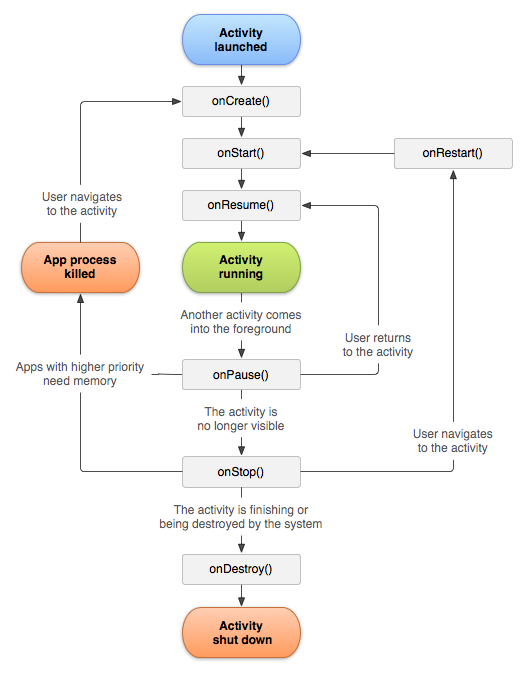
\includegraphics[width=.9\linewidth]{./pic/activityLifeCycle.png}
\end{itemize}
\section{Activity生命周期相关函数说明}
\label{sec-1-1}
\begin{itemize}
\item (1) onCreate()是activity正在被创建,也就是说此时的UI操作不会更新UI,比如setText()操作,所以此时在子线程调用setText()不会报线程错误。详解可见Android子线程更新View的探索,在这个方法内我们可以做一些初始化工作。
\item (2) onRestart()需要注意的是:activity正在重新启动,一般情况下,activity从不可见状态到可见状态,onRestart()才会被调用,但是一定要注意的是一般来说这是用户行为导致activity不可见的时候,此时变为可见的时候才会调用onRestart(),这里所说的用户行为就是用户按home键,或者进入“新”的activity。这样的操作会使activity先执行onPause(),后执行onStop(),这样回到这个activity会调用onRestart()。为什么我这里强调说用户行为导致的不可见状态,等下我会说。。。。
\item (3) onStart()的时候,activity才可见,但是没有出现在前台,无法与用户交互
\item (4) onResume()的时候,activity已经可见,并且出现在前台开始活动,与onStart()相比,activity都已经可见,但是onStart()的时候activity还在后台,onResume()才显示在前台
\item (5) onPause()主要注意的是:此时的activity正在被停止,接下来马上调用onStop()。特殊情况下快速回到该activity,onStop()不会执行,会去执行onResume()。
\begin{itemize}
\item \uline{一般在这个生命周期内做存储数据、停止动画工作,但不能太耗时。}
\item 为什么特殊强调呢,因为该activity的onPause()执行完了,才回去执行新的activity的onResume(),一旦耗时,必然会拖慢新的activity的显示。
\end{itemize}
\item (6) onStop():此时的activity即将停止。在这里可以做稍微重量级的操作,同样也不能耗时。
\item (7) onDestroy():此时的activity即将被回收,在这里会做一些回收工作和最终资源释放。
\end{itemize}
\subsection{在这里着重讲解一下onStart与onResume,onPause与onStop区别}
\label{sec-1-1-1}
onStart与onResume两种状态虽都可见,但onStart时还无法与用户交互,并未获得焦点。onResume时页面已获得焦点,可与用户交互;onPause时页面还在前台,只不过页面已失去焦点,无法与用户交互了,onStop时已不可见了。

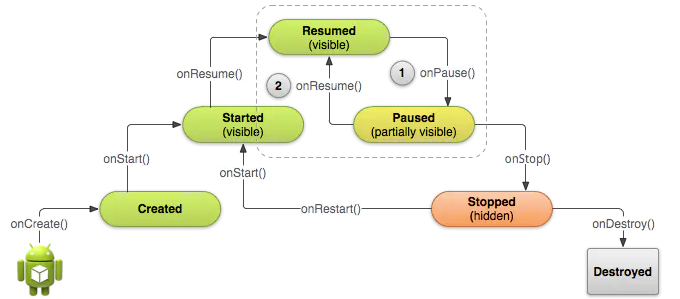
\includegraphics[width=.9\linewidth]{./pic/states.png}

activity四个状态所在的生命周期:

\begin{itemize}
\item Running状态:一个新的Activity启动入栈后,它在屏幕最前端,处于栈的最顶端,此时它处于可见并可和用户交互的激活状态。
\item Paused状态:依旧在用户可见状态,但是界面焦点已经失去,此Activity无法与用户进行交互。当Activity被另一个透明或者Dialog样式的Activity覆盖时的状态。此时它依然与窗口管理器保持连接,系统继续维护其内部状态,它仍然可见,但它已经失去了焦点,故不可与用户交互。所以就解释为什么启动一个dialogActivity或者透明Activity时,原Activity只执行了onPause生命周期,并未执行onStop
\item Stopped状态:用户看不到当前界面,也无法与用户进行交互 完全被覆盖。当Activity不可见时,Activity处于Stopped状态。当Activity处于此状态时,一定要保存当前数据和当前的UI状态,否则一旦Activity退出或关闭时,当前的数据和UI状态就丢失了。
\item Killed状态:Activity被杀掉以后或者被启动以前,处于Killed状态。这是Activity已从Activity堆栈中移除,需要重新启动才可以显示和使用。
\item 4种状态中,Running状态和Paused状态是可见的,Stopped状态和Killed状态时不可见的。
\end{itemize}

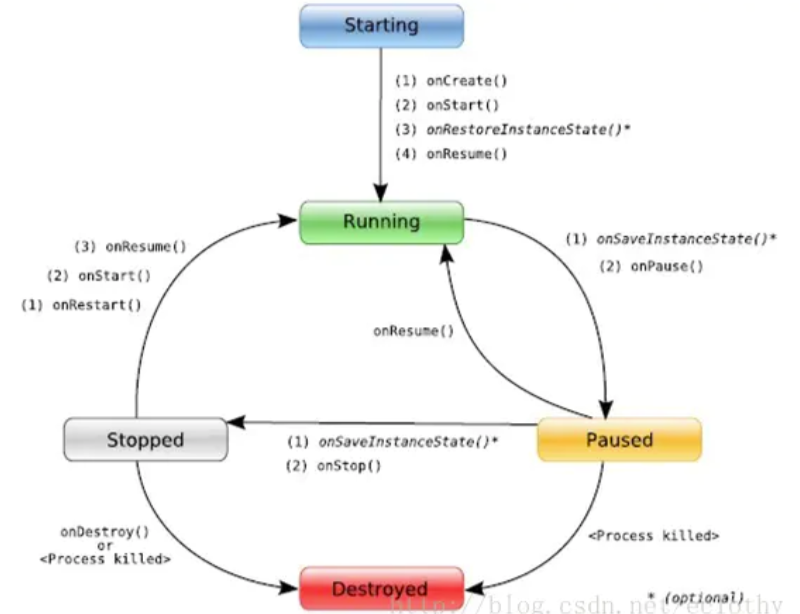
\includegraphics[width=.9\linewidth]{./pic/func.png}

\section{Activity注意事项}
\label{sec-1-2}
\begin{itemize}
\item Activity中所有和状态相关的回调函数:
\end{itemize}

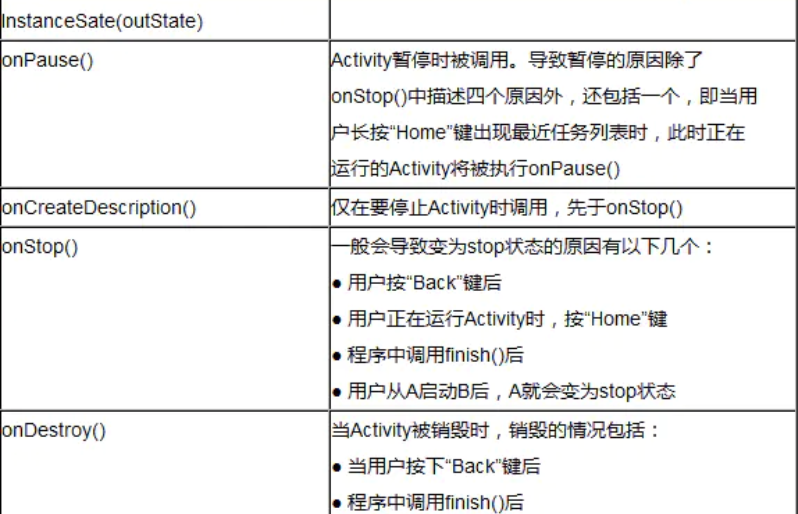
\includegraphics[width=.9\linewidth]{./pic/one.png}

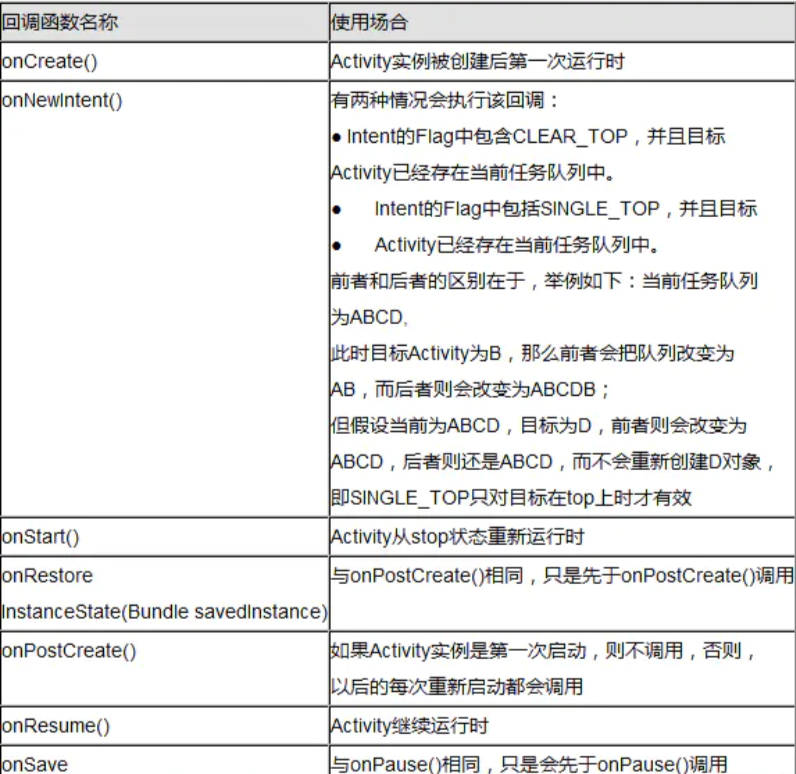
\includegraphics[width=.9\linewidth]{./pic/two.png}

\includegraphics[width=.9\linewidth]{./pic/activityLifecyleCallbacks.png}

\begin{itemize}
\item 在这里我会特别提出一个point,就是异常情况下activity被杀死,而后被重新创建的情况。

\begin{figure}[htb]
\centering
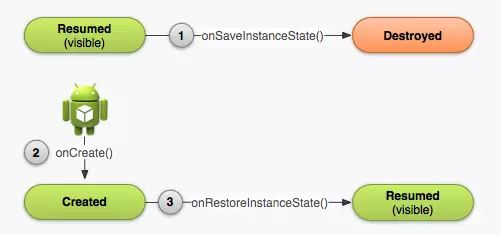
\includegraphics[width=.9\linewidth]{./pic/recreateActivity.png}
\caption{异常情况下activity的重建过程}
\end{figure}

\item 这张图非常重要,可以帮我们解决异常情况下activity如何正常回复的问题
\item 当系统停止activity时,它会调用onSaveInstanceState()(过程1),如果activity被销毁了,但是需要创建同样的实例,系统会把过程1中的状态数据传给onCreate()和onRestoreInstanceState(),所以我们要在onSaveInstanceState()内做保存参数的动作,在onRestoreInstanceState()做获取参数的动作。
\begin{minted}[frame=lines,fontsize=\scriptsize,linenos=false]{java}
// Save Activity State
static final String STATE_SCORE = "playerScore";
static final String STATE_LEVEL = "playerLevel";
@Override
public void onSaveInstanceState(Bundle savedInstanceState) {
    savedInstanceState.putInt(STATE_SCORE, mCurrentScore); // Save the user's current game state
    savedInstanceState.putInt(STATE_LEVEL, mCurrentLevel);
    super.onSaveInstanceState(savedInstanceState); // Always call the superclass so it can save the view hierarchy state
}
\end{minted}
\item 获取参数操作:
\begin{minted}[frame=lines,fontsize=\scriptsize,linenos=false]{java}
// onCreate() 方法
@Override
protected void onCreate(Bundle savedInstanceState) {
    super.onCreate(savedInstanceState); // Always call the superclass first
    if (savedInstanceState != null) { // Check whether we're recreating a previously destroyed instance
        mCurrentScore = savedInstanceState.getInt(STATE_SCORE); // Restore value of members from saved state
        mCurrentLevel = savedInstanceState.getInt(STATE_LEVEL);
    } else  // Probably initialize members with default values for a new instance
}
\end{minted}
\item 也可以
\begin{minted}[frame=lines,fontsize=\scriptsize,linenos=false]{java}
// onRestoreInstanceState()方法
public void onRestoreInstanceState(Bundle savedInstanceState) {
    super.onRestoreInstanceState(savedInstanceState); // Always call the superclass so it can restore the view hierarchy
    mCurrentScore = savedInstanceState.getInt(STATE_SCORE); // Restore state members from saved instance
    mCurrentLevel = savedInstanceState.getInt(STATE_LEVEL);
}
\end{minted}
\end{itemize}

\section{一些特殊的方法}
\label{sec-1-3}
\subsection{onWindowFocusChanged()}
\label{sec-1-3-1}
\begin{itemize}
\item 在Activity窗口获得或失去焦点时被调用并且当Activity被创建时是在onResume之后被调用,当Activity被覆盖或者退居后台或者当前Activity退出时,它是在onPause之后被调用(在这个方法中可以view已经绘制完成,可以获取view的宽高等属性)
\end{itemize}
\subsection{onSaveInstanceState()}
\label{sec-1-3-2}
\begin{itemize}
\item (1)在Activity被覆盖或退居后台之后,系统资源不足将其杀死,此方法会被调用;
\item (2)在用户改变屏幕方向时,此方法会被调用;
\item (3)在当前Activity跳转到其他Activity或者按Home键回到主屏,自身退居后台时,此方法会被调用。
\item 第一种情况我们无法保证什么时候发生,系统根据资源紧张程度去调度;
\item 第二种是屏幕翻转方向时,系统先销毁当前的Activity,然后再重建一个新的,调用此方法时,我们可以保存一些临时数据;
\item 第三种情况系统调用此方法是为了保存当前窗口各个View组件的状态。
\item onSaveInstanceStat()e的调用顺序是在onStop()之前。(android3.0之前:在onPause之前调用,在3.0之后,在onPause之后调用)
\end{itemize}
\subsection{onRestoreInstanceState()}
\label{sec-1-3-3}
\begin{itemize}
\item 有的人说这个方法和onSaveInstanceState是一对,其实不然,
\item (1)在Activity被覆盖或退居后台之后,系统资源不足将其杀死,然后用户又回到了此Activity,此方法会被调用;
\item (2)在用户改变屏幕方向时,重建的过程中,此方法会被调用。
\item 我们可以重写此方法,以便可以恢复一些临时数据。
\item onRestoreInstanceState的调用顺序是在onStart之后。
\item 在当前Activity跳转到其他Activity或者按Home键回到主屏,自身退居后台时:onRestoreInstanceState不会调用,但是onSaveInstanceState会调用,这点就是区别(验证一下)
\end{itemize}
\subsection{注意一下两个函数在生命周期中的调用顺序}
\label{sec-1-3-4}
\begin{minted}[frame=lines,fontsize=\scriptsize,linenos=false]{java}
onCreate()
onStart()
onRestoreInstanceState() // onStart() 之后恢复数据
onResume()
onPause()
onSaveInstanceState()    // onStop() 之前保存数据
onStop()
onDestory()
\end{minted}
\section{最后的总结}
\label{sec-1-4}
\begin{itemize}
\item 当Activity被系统撤销后重新建立时,保存以及恢复数据的函数调用顺序是:
\begin{itemize}
\item onSaveInstanceState(保存数据) ----> onStop() 
----> onCreate(恢复数据allstate) ----> onStart() ----> onRestoryInstanceState(恢复数据HierarchyState) ---> onResume()
\end{itemize}
\item 如果要取消切换屏幕方法重建activity,可以配置configChanges属性:当支持的最小sdk版本大于android4.0需要设置这个属性)
\begin{itemize}
\item 其中Bundle数据会传到onCreate()(不一定有数据)和onRestoreInstanceState()(一定有数据)。
\item Activity在manifest.xml文件中可以指定参数android:ConfigChanges,用于捕获手机状态的改变
\item 在Activity中添加了android:configChanges属性,在当所指定属性(Configuration Changes)发生改变时,通知程序调用onConfigurationChanged()函数。
\end{itemize}
\item 设置方法:将下列字段用“|”符号分隔开,例如:“locale|navigation|orientation” 
\begin{itemize}
\item “mcc“ 移动国家号码,由三位数字组成,每个国家都有自己独立的MCC,可以识别手机用户所属国家。
\item “mnc“ 移动网号,在一个国家或者地区中,用于区分手机用户的服务商。
\item “locale“ 所在地区发生变化。
\item “touchscreen“ 触摸屏已经改变。(这不应该常发生。)
\item “keyboard“ 键盘模式发生变化,例如:用户接入外部键盘输入。
\item “keyboardHidden“ 用户打开手机硬件键盘
\item “navigation“ 导航型发生了变化。(这不应该常发生。)
\item “orientation“ 设备旋转,横向显示和竖向显示模式切换。
\item “fontScale“ 全局字体大小缩放发生改变
\end{itemize}
\item 对android:configChanges属性,一般认为有以下几点:(这里面的次数是怎么数的,还没有搞懂)
\begin{itemize}
\item 1、不设置Activity的android:configChanges时,切屏会重新调用各个生命周期,切横屏时会执行一次,切竖屏时会执行两次
\item 2、设置Activity的android:configChanges="orientation"时,切屏还是会重新调用各个生命周期,切横、竖屏时只会执行一次
\item 3、设置Activity的android:configChanges="orientation|keyboardHidden"时,切屏不会重新调用各个生命周期,只会执行onConfigurationChanged方法
\end{itemize}
\item 自从Android 3.2(API 13),在设置Activity的android:configChanges="orientation|keyboardHidden"后,还是一样会重新调用各个生命周期的。因为screen size也开始跟着设备的横竖切换而改变。所以,在AndroidManifest.xml里设置的MiniSdkVersion和 TargetSdkVersion属性大于等于13的情况下,如果你想阻止程序在运行时重新加载Activity,除了设置"orientation",你还必须设置"ScreenSize"。
\begin{itemize}
\item 解决方法:AndroidManifest.xml中设置
\end{itemize}
\end{itemize}
\begin{minted}[frame=lines,fontsize=\scriptsize,linenos=false]{xml}
android:configChanges="orientation|screenSize“
\end{minted}

\begin{minted}[frame=lines,fontsize=\scriptsize,linenos=false]{java}
android:configChanges="keyboardHidden|orientation|screenSize(当支持的最小sdk版本大于android4.0需要设置这个属性)"
\end{minted}

\section{他人总结}
\label{sec-1-5}
\begin{itemize}
\item 横竖屏切换时 Activity 的生命周期
\end{itemize}
1、不设置 Activity 的 android:configChanges 时,切屏会重新调用各个生命周期 默认首先销毁当前 activity,然后重新加载。如下图,当横竖屏切换时先执行 onPause/onStop 方法
\begin{minted}[frame=lines,fontsize=\scriptsize,linenos=false]{java}
onPause()
onStop()
onCreate()
onStart()
onResume()
\end{minted}
2、设置 Activity 的 android:configChanges="orientation|keyboardHidden|screenSize"时,切屏不会重新调 用各个生命周期,只会执行 onConfigurationChanged 方法。

\begin{itemize}
\item \url{https://juejin.im/post/5a18f58651882531bb6c82e2}
\item 1. 打开一个全新的activityA:
\begin{itemize}
\item onCreate() ----> onStart() ----> onResume()
\end{itemize}
\item 2. 从activity A ----> activity B(全屏):
\begin{itemize}
\item activity A 先执行: onPause()
\item 然后activity B执行: onCreate() ----> onStart() ----> onResume()
\item activity A 再执行: onStop()
\end{itemize}
\item 3. 从activity A ----> activity B(非全屏):
\begin{itemize}
\item activity A先执行: onPause()
\item 然后activity B执行: onCreate() ----> onStart() ----> onResume()
\item \textbf{activity A不会执行onStop()}
\end{itemize}
\item 4. activity B(全屏)返回到 activity A:
\begin{itemize}
\item activity B 先执行: onPause()
\item activity A: onRestart ----> onStart() ----> onResume()
\item activity B再执行: onStop() ----> onDestory()
\end{itemize}
\item 5. activity B(非全屏)返回到activity A 
\begin{itemize}
\item activity B先执行: onPause()
\item activity A: onResume()
\item activity B再执行: onStop() ----> onDestory()
\end{itemize}
\item 6. activity B返回到activity A:
\begin{itemize}
\item 如果activityA已经被销毁,activityA会重新创建,执行: onCreate() ----> onStart() ----> onResume()
\item activityB的流程不变
\end{itemize}
\item 7. activity A按home键退居后台:
\begin{itemize}
\item 同2的流程: onPause()
\end{itemize}
\item 8. 再从home返回到activity A
\begin{itemize}
\item 同4的流程: onRestart ----> onStart() ----> onResume()
\end{itemize}
\end{itemize}
\section{activity之间的数据传递: 6种方式}
\label{sec-1-6}
\subsection{使用Inten的putExtra传递}
\label{sec-1-6-1}
\begin{itemize}
\item 第一个Activity中
\begin{minted}[frame=lines,fontsize=\scriptsize,linenos=false]{java}
Intent intent = new Intent(this,TwoActivity.class);
intent.putExtra("data",str);
startActivity(intent);
\end{minted}
\item 第二个Activity
\begin{minted}[frame=lines,fontsize=\scriptsize,linenos=false]{java}
Intent intent = getIntent();
String str = intent.getStringExtra("data");
tv.setText(str);
\end{minted}
\end{itemize}
\subsection{使用Intent的Bundle传递}
\label{sec-1-6-2}
\begin{itemize}
\item 第一个Activity中
\begin{minted}[frame=lines,fontsize=\scriptsize,linenos=false]{java}
Intent intent = new Intent(MainActivity.this,TwoActivity.class);
Bundle bundle = new Bundle();
bundle.putString("data", str);
intent.putExtra("bun", bundle);
startActivity(intent);
\end{minted}
\item 第二个Activity
\begin{minted}[frame=lines,fontsize=\scriptsize,linenos=false]{java}
Intent intent = getIntent();
Bundle bundle = intent.getBundleExtra("bun");
String str = bundle.getString("data");
tv.setText(str);
\end{minted}
\end{itemize}
\subsection{使用Activity销毁时传递数据}
\label{sec-1-6-3}
\begin{itemize}
\item 第一个Activity中
\begin{minted}[frame=lines,fontsize=\scriptsize,linenos=false]{java}
Intent intent = new Intent(MainActivity.this,TwoActivity.class);
startActivityForResult(intent, 11);
protected void onActivityResult(int requestCode, int resultCode, Intent data) {
    super.onActivityResult(requestCode, resultCode, data);
    String str = data.getStringExtra("data");
    tvOne.setText(str);
}
\end{minted}
\item 第二个Activity
\begin{minted}[frame=lines,fontsize=\scriptsize,linenos=false]{java}
Intent intent = new Intent();
intent.putExtra("data", edtOne.getText().toString().trim());
setResult(3, intent);
finish();
\end{minted}
\end{itemize}
\subsection{SharedPreferences传递数据}
\label{sec-1-6-4}
\begin{itemize}
\item 第一个Activity中
\begin{minted}[frame=lines,fontsize=\scriptsize,linenos=false]{java}
SharedPreferences sp = this.getSharedPreferences("info", 1);
Editor edit = sp.edit();
edit.putString("data", str);
edit.commit();
Intent intent = new Intent(MainActivity.this,TwoActivity.class);
startActivity(intent);
\end{minted}
\item 第二个Activity
\begin{minted}[frame=lines,fontsize=\scriptsize,linenos=false]{java}
SharedPreferences sp = this.getSharedPreferences("info", 1);
tv.setText(sp.getString("data", ""));
\end{minted}
\end{itemize}
\subsection{使用序列化对象Seriazable}
\label{sec-1-6-5}
\begin{itemize}
\item 这里需要建一个工具类
\end{itemize}
\begin{minted}[frame=lines,fontsize=\scriptsize,linenos=false]{java}
import java.io.Serializable;
class DataBean implements Serializable {
    private String name;
    private String sex;
    public String getName() {
        return name;
    }
    public void setName(String name) {
        this.name = name;
    }
    public String getSex() {
        return sex;
    }
    public void setSex(String sex) {
        this.sex = sex;
    }
}
\end{minted}
\begin{itemize}
\item 第一个Activity中
\begin{minted}[frame=lines,fontsize=\scriptsize,linenos=false]{java}
Intent intent = new Intent(MainActivity.this,TwoActivity.class);
DataBean bean = new DataBean();
bean.setName("啦啦");
bean.setSex("男");
intent.putExtra("key", bean);
startActivity(intent);
\end{minted}
\item 第二个Activity
\begin{minted}[frame=lines,fontsize=\scriptsize,linenos=false]{java}
Intent intent = getIntent();
//反序列化数据对象
Serializable se = intent.getSerializableExtra("key");
if (se instanceof DataBean){
    //获取到携带数据的DataBean对象db
    DataBean db = (DataBean) se;
    tv.setText(db.getName()+"==="+db.getSex());
}
\end{minted}
\end{itemize}
\subsection{使用静态变量传递数据}
\label{sec-1-6-6}
\begin{itemize}
\item 第一个Activity中
\begin{minted}[frame=lines,fontsize=\scriptsize,linenos=false]{java}
Intent intent = new Intent(MainActivity.this,TwoActivity.class);
TwoActivity.name="牛逼";
TwoActivity.str="你说";
startActivity(intent);
\end{minted}
\item 第二个Activity
\begin{minted}[frame=lines,fontsize=\scriptsize,linenos=false]{java}
protected static String name;
protected static String str;
tv.setText(str+name);
\end{minted}
\end{itemize}
\subsection{剪切板,利用系统剪切板服务,稍偏}
\label{sec-1-6-7}
\begin{itemize}
\item 第一个Activity中
\begin{minted}[frame=lines,fontsize=\scriptsize,linenos=false]{java}
ClipboardManager clipboardManager = (ClipboardManager) getSystemService(Context.CLIPBOARD_SERVICE);
String name = "AHuier";
clipboardManager.setText(name);
Intent intent = new Intent(IntentDemo.this, Other.class);
startActivity(intent);
\end{minted}
\item 第二个Activity
\begin{minted}[frame=lines,fontsize=\scriptsize,linenos=false]{java}
ClipboardManager clipboardManager = (ClipboardManager) getSystemService(Context.CLIPBOARD_SERVICE);
String msgString = clipboardManager.getText().toString();
textView.setText(msgString);
\end{minted}
\item 利用剪切板传递复杂的数据,如对象,略
\end{itemize}


\chapter{Fragment生命周期探讨}
\label{sec-2}
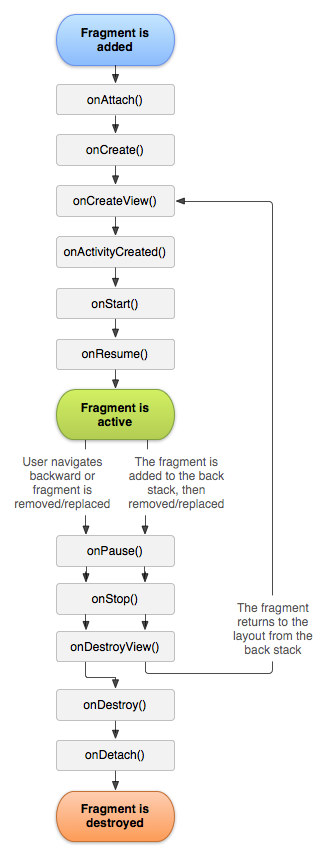
\includegraphics[width=.9\linewidth]{./pic/fragmentlifecycle.png}
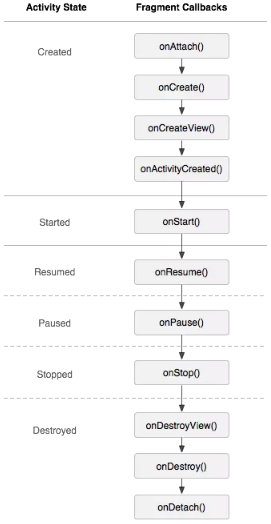
\includegraphics[width=.9\linewidth]{./pic/lifecyclecompare.png}

\begin{itemize}
\item Fragment基本类,生命周期如下:
\begin{minted}[frame=lines,fontsize=\scriptsize,linenos=false]{java}
void onAttach(Context context)
void onCreate(Bundle savedInstanceState)
View onCreateView(LayoutInflater inflater, ViewGroup container, Bundle savedInstanceState)
void onActivityCreated(Bundle savedInstanceState)
void onStart()
void onResume()
void onPause()
void onStop()
void onDestroyView()
void onDestroy()
void onDetach()
\end{minted}
\end{itemize}

\section{首先需要提出的一些points:}
\label{sec-2-1}
\begin{itemize}
\item Fragment是直接从Object继承的,而Activity是Context的子类。因此我们可以得出结论:Fragment不是Activity的扩展。但是与Activity一样,在我们使用Fragment的时候我们总会扩展Fragment(或者是她的子类),并可以通过子类更改她的行为。
\item 使用Fragment时,必要构建一个无参构造函数,系统会默认带。但一但写有参构造函数,就必要构建无参构造函数。一般来说我们传参数给Fragment,会通过bundle,而不会用构造方法传,代码如下:
\begin{minted}[frame=lines,fontsize=\scriptsize,linenos=false]{java}
public static MyFragment newInstance(int index){  
    MyFragment mf = new MyFragment();  
    Bundle args = new Bundle();  
    args.putInt("index",index);  
    mf.setArguments(args);  
    return mf;  
}
\end{minted}
\end{itemize}
\section{生命周期}
\label{sec-2-2}
\begin{itemize}
\item onAttach():onAttach()回调将在Fragment与其Activity关联之后调用。需要使用Activity的引用或者使用Activity作为其他操作的上下文,将在此回调方法中实现。
\begin{itemize}
\item 将Fragment附加到Activity以后,就无法再次调用setArguments()--除了在最开始,无法向初始化参数添加内容。
\end{itemize}
\item onCreate(Bundle savedInstanceState):此时的Fragment的onCreate()回调时,该fragmet还没有获得Activity的onCreate()已完成的通知,所以不能将依赖于Activity视图层次结构存在性的代码放入此回调方法中。在onCreate()回调方法中,我们应该尽量避免耗时操作。此时的bundle就可以获取到activity传来的参数
\begin{minted}[frame=lines,fontsize=\scriptsize,linenos=false]{java}
@Override
public void onCreate(Bundle savedInstanceState) {  
        super.onCreate(savedInstanceState);  
        Bundle args = getArguments();  
        if (args != null) {  
            mLabel = args.getCharSequence("label", mLabel);  
        }  
    }
\end{minted}
\item onCreateView()
\begin{minted}[frame=lines,fontsize=\scriptsize,linenos=false]{java}
onCreateView(LayoutInflater inflater, ViewGroup container, Bundle savedInstanceState)
\end{minted}
\begin{itemize}
\item 其中的Bundle为状态包与上面的bundle不一样。
\item 不要将视图层次结构附加到传入的ViewGroup父元素中,该关联会自动完成。如果在此回调中将碎片的视图层次结构附加到父元素,很可能会出现异常。
\item 这句话什么意思呢?就是不要把初始化的view视图主动添加到container里面,以为这会系统自带,所以inflate函数的第三个参数必须填false,而且不能出现container.addView(v)的操作。
\end{itemize}
\begin{minted}[frame=lines,fontsize=\scriptsize,linenos=false]{java}
View v = inflater.inflate(R.layout.hello_world, container, false);
\end{minted}
\item onActivityCreated()
\begin{itemize}
\item onActivityCreated()回调会在Activity完成其onCreate()回调之后调用。在调用onActivityCreated()之前,Activity的视图层次结构已经准备好了,这是在用户看到用户界面之前你可对用户界面执行的最后调整的地方。
\item 如果Activity和她的Fragment是从保存的状态重新创建的,此回调尤其重要,也可以在这里确保此Activity的其他所有Fragment已经附加到该Activity中了
\end{itemize}
\item Fragment与Activity相同生命周期调用:接下来的onStart(), onResume(), onPause(), onStop()回调方法将和Activity的回调方法进行绑定,也就是说与Activity中对应的生命周期相同,因此不做过多介绍。
\item onDestroyView():该回调方法在视图层次结构与Fragment分离之后调用。
\item onDestroy():不再使用Fragment时调用。(备注:Fragment仍然附加到Activity并任然可以找到,但是不能执行其他操作)
\item onDetach():Fragment生命周期最后回调函数,调用后,Fragment不再与Activity绑定,释放资源。
\end{itemize}

\section{Fragment每个生命周期方法的意义、作用}
\label{sec-2-3}
\begin{itemize}
\item onAttach()
\begin{itemize}
\item 执行该方法时,Fragment与Activity已经完成绑定,该方法有一个Activity类型的参数,代表绑定的Activity,这时候你可以执行诸如mActivity = activity的操作。
\end{itemize}
\item onCreate()
\begin{itemize}
\item 初始化Fragment。可通过参数savedInstanceState获取之前保存的值。
\end{itemize}
\item onCreateView()
\begin{itemize}
\item 初始化Fragment的布局。加载布局和findViewById的操作通常在此函数内完成,但是不建议执行耗时的操作,比如读取数据库数据列表。
\end{itemize}
\item onActivityCreated()
\begin{itemize}
\item 执行该方法时,与Fragment绑定的Activity的onCreate方法已经执行完成并返回,在该方法内可以进行与Activity交互的UI操作,所以在该方法之前Activity的onCreate方法并未执行完成,如果提前进行交互操作,会引发空指针异常。
\end{itemize}
\item onStart()
\begin{itemize}
\item 执行该方法时,Fragment由不可见变为可见状态。
\end{itemize}
\item onResume()
\begin{itemize}
\item 执行该方法时,Fragment处于活动状态,用户可与之交互。
\end{itemize}
\item onPause()
\begin{itemize}
\item 执行该方法时,Fragment处于暂停状态,但依然可见,用户不能与之交互。
\end{itemize}
\item onSaveInstanceState()
\begin{itemize}
\item 保存当前Fragment的状态。该方法会自动保存Fragment的状态,比如EditText键入的文本,即使Fragment被回收又重新创建,一样能恢复EditText之前键入的文本。
\end{itemize}
\item onStop()
\begin{itemize}
\item 执行该方法时,Fragment完全不可见。
\end{itemize}
\item onDestroyView()
\begin{itemize}
\item 销毁与Fragment有关的视图,但未与Activity解除绑定,依然可以通过onCreateView方法重新创建视图。通常在ViewPager+Fragment的方式下会调用此方法。
\end{itemize}
\item onDestroy()
\begin{itemize}
\item 销毁Fragment。通常按Back键退出或者Fragment被回收时调用此方法。
\end{itemize}
\item onDetach()
\begin{itemize}
\item 解除与Activity的绑定。在onDestroy方法之后调用。
\end{itemize}
\item setUserVisibleHint()
\begin{itemize}
\item 设置Fragment可见或者不可见时会调用此方法。在该方法里面可以通过调用getUserVisibleHint()获得Fragment的状态是可见还是不可见的,如果可见则进行懒加载操作。
\end{itemize}
\end{itemize}
\section{Fragment生命周期执行流程}
\label{sec-2-4}
\begin{itemize}
\item 1、Fragment创建
\begin{itemize}
\item setUserVisibleHint() ----> onAttach() ----> onCreate() ----> onCreateView() ----> onActivityCreated() ----> onStart() ----> onResume()
\end{itemize}
\item 2、Fragment变为不可见状态(锁屏、回到桌面、被Activity完全覆盖)
\begin{itemize}
\item onPause() ----> onSaveInstanceState() ----> onStop()
\end{itemize}
\item 3、Fragment变为部分可见状态(打开Dialog样式的Activity)
\begin{itemize}
\item onPause() ----> onSaveInstanceState()
\end{itemize}
\item 4、Fragment由不可见变为活动状态
\begin{itemize}
\item onStart() ----> OnResume()
\end{itemize}
\item 5、Fragment由部分可见变为活动状态
\begin{itemize}
\item onResume()
\end{itemize}
\item 6、Fragment退出
\begin{itemize}
\item onPause() ----> onStop() ----> onDestroyView() ----> onDestroy() ----> onDetach()
\item (注意退出不会调用onSaveInstanceState方法,因为是人为退出,没有必要再保存数据)
\end{itemize}
\item 7、Fragment被回收又重新创建
\begin{itemize}
\item 被回收执行: onPause() ----> onSaveInstanceState() ----> onStop() ----> onDestroyView() ----> onDestroy() ----> onDetach()
\item 重新创建执行: onAttach() ----> onCreate() ----> onCreateView() ----> onActivityCreated() ----> onStart() ----> onResume() ----> setUserVisibleHint()
\end{itemize}
\item 横竖屏切换
\begin{itemize}
\item 与Fragment被回收又重新创建一样。
\end{itemize}
\end{itemize}
\section{onHiddenChanged的回调时机}
\label{sec-2-5}
\begin{itemize}
\item 当使用add()+show(),hide()跳转新的Fragment时,旧的Fragment回调onHiddenChanged(),不会回调onStop()等生命周期方法,而新的Fragment在创建时是不会回调onHiddenChanged(),这点要切记。
\end{itemize}
\section{FragmentPagerAdapter+ViewPager的注意事项}
\label{sec-2-6}
\begin{itemize}
\item 1、 使用FragmentPagerAdapter+ViewPager时,切换回上一个Fragment页面时(已经初始化完毕),不会回调任何生命周期方法以及onHiddenChanged(),只有setUserVisibleHint(boolean isVisibleToUser)会被回调,所以如果你想进行一些懒加载,需要在这里处理。
\item 2、 在给ViewPager绑定FragmentPagerAdapter时,new FragmentPagerAdapter(fragmentManager)的FragmentManager,一定要保证正确,如果ViewPager是Activity内的控件,则传递getSupportFragmentManager(),如果是Fragment的控件中,则应该传递getChildFragmentManager()。只要记住ViewPager内的Fragments是当前组件的子Fragment这个原则即可。
\item 3、 你不需要考虑在“内存重启”的情况下,去恢复的Fragments的问题,因为FragmentPagerAdapter已经帮我们处理啦。
\end{itemize}
\section{setUserVisibleHint()不调用的问题}
\label{sec-2-7}
\begin{itemize}
\item 通常情况下都是因为PagerAdapter不是FragmentPagerAdapter造成的,FragmentPagerAdapter内部实现了对setUserVisibleHint()方法的调用,所以需要懒加载的结构最好使用FragmentPagerAdapter +Fragment的结构,少用PagerAdapter。
\end{itemize}
\section{详细细节}
\label{sec-2-8}
\begin{itemize}
\item 我们这里举个例子来理解Fragment生命周期方法。功能如下:共有两个Fragment:F1和F2,F1在初始化时就加入Activity,点击F1中的按钮调用replace替换为F2。
\item 当F1在Activity的onCreate()中被添加时,日志如下:
\end{itemize}
\begin{minted}[frame=lines,fontsize=\scriptsize,linenos=false]{java}
MainActivity: onCreate() BEGIN
MainActivity: onCreate() END

MainActivity: onStart() BEGIN
Fragment1: onAttach() BEGIN 
Fragment1: onAttach() END
MainActivity: onAttachFragment() BEGIN
MainActivity: onAttachFragment() END
Fragment1: onCreate() BEGIN
Fragment1: onCreate() END
Fragment1: onCreateView()
Fragment1: onViewCreated() BEGIN
Fragment1: onViewCreated() END
Fragment1: onActivityCreated() BEGIN
Fragment1: onActivityCreated() END
Fragment1: onStart() BEGIN
Fragment1: onStart() END
MainActivity: onStart() END

MainActivity: onPostCreate() BEGIN
MainActivity: onPostCreate() END
MainActivity: onResume() BEGIN
MainActivity: onResume() END
MainActivity: onPostResume() BEGIN
Fragment1: onResume() BEGIN
Fragment1: onResume() END
MainActivity: onPostResume() END
MainActivity: onAttachedToWindow() BEGIN
MainActivity: onAttachedToWindow() END
\end{minted}
\begin{itemize}
\item 可以看出:
\begin{itemize}
\item Fragment的onAttach()->onCreate()->onCreateView()->onActivityCreated()->onStart()都是在Activity的onStart()中调用的。
\item Fragment的onResume()在Activity的onResume()之后调用。
\end{itemize}
\item 接下去分两种情况,分别是不加addToBackStack()和加addToBackStack()。
\begin{itemize}
\item 1、当点击F1的按钮,调用replace()替换为F2,且不加addToBackStack()时,日志如下:
\end{itemize}
\end{itemize}
\begin{minted}[frame=lines,fontsize=\scriptsize,linenos=false]{java}
Fragment2: onAttach() BEGIN
Fragment2: onAttach() END
MainActivity: onAttachFragment() BEGIN
MainActivity: onAttachFragment() END
Frag    2: onCreate() BEGIN
Frag    2: onCreate() END
Fragment1: onPause() BEGIN
Fragment1: onPause() END
Fragment1: onStop() BEGIN
Fragment1: onStop() END
Fragment1: onDestroyView() BEGIN
Fragment1: onDestroyView() END
Fragment1: onDestroy() BEGIN
Fragment1: onDestroy() END
Fragment1: onDetach() BEGIN
Fragment1: onDetach() END
Frag    2: onCreateView()
Frag    2: onViewCreated() BEGIN
Frag    2: onViewCreated() END
Frag    2: onActivityCreated() BEGIN
Frag    2: onActivityCreated() END
Frag    2: onStart() BEGIN
Frag    2: onStart() END
Frag    2: onResume() BEGIN
Frag    2: onResume() END
\end{minted}
\begin{itemize}
\item 可以看到,F1最后调用了onDestroy()和onDetach()。
\item 2、当点击F1的按钮,调用replace()替换为F2,且加addToBackStack()时,日志如下:
\end{itemize}
\begin{minted}[frame=lines,fontsize=\scriptsize,linenos=false]{java}
Frag    2: onAttach() BEGIN
Frag    2: onAttach() END
MainActivity: onAttachFragment() BEGIN
MainActivity: onAttachFragment() END
Frag    2: onCreate() BEGIN
Frag    2: onCreate() END
Fragment1: onPause() BEGIN
Fragment1: onPause() END
Fragment1: onStop() BEGIN
Fragment1: onStop() END
Fragment1: onDestroyView() BEGIN
Fragment1: onDestroyView() END
Frag    2: onCreateView()
Frag    2: onViewCreated() BEGIN
Frag    2: onViewCreated() END
Frag    2: onActivityCreated() BEGIN
Frag    2: onActivityCreated() END
Frag    2: onStart() BEGIN
Frag    2: onStart() END
Frag    2: onResume() BEGIN
Frag    2: onResume() END
\end{minted}
\begin{itemize}
\item 可以看到,F1被替换时,最后只调到了onDestroyView(),并没有调用onDestroy()和onDetach()。当用户点返回按钮回退事务时,F1会调onCreateView()->onStart()->onResume(),因此在Fragment事务中加不加addToBackStack()会影响Fragment的生命周期。
\item FragmentTransaction有一些基本方法,下面给出调用这些方法时,Fragment生命周期的变化:
\begin{itemize}
\item add(): onAttach()->…->onResume()。
\item remove(): onPause()->…->onDetach()。
\item replace(): 相当于旧Fragment调用remove(),新Fragment调用add()。
\item show(): 不调用任何生命周期方法,调用该方法的前提是要显示的Fragment已经被添加到容器,只是纯粹把Fragment UI的setVisibility为true。
\item hide(): 不调用任何生命周期方法,调用该方法的前提是要显示的Fragment已经被添加到容器,只是纯粹把Fragment UI的setVisibility为false。
\item detach(): onPause()->onStop()->onDestroyView()。UI从布局中移除,但是仍然被FragmentManager管理。
\item attach(): onCreateView()->onStart()->onResume()。
\end{itemize}
\end{itemize}

\section{Fragment基础知识}
\label{sec-2-9}
\begin{itemize}
\item 核心的类有:
\begin{itemize}
\item Fragment:Fragment的基类,任何创建的Fragment都需要继承该类。
\item FragmentManager:管理和维护Fragment。他是抽象类,具体的实现类是FragmentManagerImpl。
\item FragmentTransaction:对Fragment的添加、删除等操作都需要通过事务方式进行。他是抽象类,具体的实现类是BackStackRecord。
\end{itemize}
\item Nested Fragment(Fragment内部嵌套Fragment的能力)是Android 4.2提出的,support-fragment库可以兼容到1.6。通过getChildFragmentManager()能够获得管理子Fragment的FragmentManager,在子Fragment中可以通过getParentFragment()获得父Fragment。
\item 这里给出Fragment最基本的使用方式。首先,创建继承Fragment的类,名为Fragment1:
\end{itemize}
\begin{minted}[frame=lines,fontsize=\scriptsize,linenos=false]{java}
public class Fragment1 extends Fragment {
    private static String ARG_PARAM = "param_key";
    private Activity mActivity; // 
    private String mParam;
    public static Fragment1 newInstance(String str) {
        Fragment1 frag = new Fragment1();
        Bundle bundle = new Bundle();
        bundle.putString(ARG_PARAM, str);
        fragment.setArguments(bundle);   //设置参数
        return fragment;
    }
    public void onAttach(Context context) {
        mActivity = (Activity) context;
        mParam = getArguments().getString(ARG_PARAM);  //获取参数
    }
    public View onCreateView(LayoutInflater inflater, ViewGroup container, Bundle savedInstanceState) {
        View root = inflater.inflate(R.layout.fragment_1, container, false);
        TextView view = root.findViewById(R.id.text);
        view.setText(mParam);
        return root;
    }
}
\end{minted}
\begin{itemize}
\item Fragment有很多可以复写的方法,其中最常用的就是onCreateView(),该方法返回Fragment的UI布局,需要注意的是inflate()的第三个参数是false,因为在Fragment内部实现中,会把该布局添加到container中,如果设为true,那么就会重复做两次添加,则会抛如下异常:
\end{itemize}
\begin{minted}[frame=lines,fontsize=\scriptsize,linenos=false]{java}
Caused by: java.lang.IllegalStateException: The specified child already has a parent. You must call removeView() on the child's parent first.
\end{minted}
\begin{itemize}
\item 如果在创建Fragment时要传入参数,必须要通过setArguments(Bundle bundle)方式添加,而不建议通过为Fragment添加带参数的构造函数,因为通过setArguments()方式添加,在由于内存紧张导致Fragment被系统杀掉并恢复(re-instantiate)时能保留这些数据。官方建议如下:
\end{itemize}
\begin{minted}[frame=lines,fontsize=\scriptsize,linenos=false]{java}
It is strongly recommended that subclasses do not have other constructors with parameters, since these constructors will not be called when the fragment is re-instantiated.
\end{minted}
\begin{itemize}
\item 我们可以在Fragment的onAttach()中通过getArguments()获得传进来的参数,并在之后使用这些参数。如果要获取Activity对象,不建议调用getActivity(),而是在onAttach()中将Context对象强转为Activity对象。
\item 创建完Fragment后,接下来就是把Fragment添加到Activity中。在Activity中添加Fragment的方式有两种:
\begin{itemize}
\item 静态添加:在xml中通过<fragment>的方式添加,缺点是一旦添加就不能在运行时删除。
\item 动态添加:运行时添加,这种方式比较灵活,因此建议使用这种方式。
\begin{itemize}
\item 这里只给出动态添加的方式。首先Activity需要有一个容器存放Fragment,一般是FrameLayout,因此在Activity的布局文件中加入FrameLayout:
\end{itemize}
\end{itemize}
\end{itemize}
\begin{minted}[frame=lines,fontsize=\scriptsize,linenos=false]{xml}
<FrameLayout
    android:id="@+id/container"
    android:layout_width="match_parent"
    android:layout_height="match_parent"
/>
\end{minted}
\begin{itemize}
\item 然后在onCreate()中,通过以下代码将Fragment添加进Activity中。
\end{itemize}
\begin{minted}[frame=lines,fontsize=\scriptsize,linenos=false]{java}
if (bundle == null) {
    getSupportFragmentManager().beginTransaction()
        .add(R.id.container, Fragment1.newInstance("hello world"), "f1")
        //.addToBackStack("fname")
        .commit();
}
\end{minted}
\begin{itemize}
\item Fragment有一个常见的问题,即Fragment重叠问题,这是由于Fragment被系统杀掉,并重新初始化时再次将fragment加入activity,因此通过在外围加if语句能判断此时是否是被系统杀掉并重新初始化的情况。
\item Fragment有个常见的异常:
\end{itemize}
\begin{minted}[frame=lines,fontsize=\scriptsize,linenos=false]{java}
java.lang.IllegalStateException: Can not perform this action after onSaveInstanceState
    at android.support.v4.app.FragmentManagerImpl.checkStateLoss(FragmentManager.java:1341)
    at android.support.v4.app.FragmentManagerImpl.enqueueAction(FragmentManager.java:1352)
    at android.support.v4.app.BackStackRecord.commitInternal(BackStackRecord.java:595)
    at android.support.v4.app.BackStackRecord.commit(BackStackRecord.java:574)
\end{minted}
\begin{itemize}
\item 该异常出现的原因是:commit()在onSaveInstanceState()后调用。首先,onSaveInstanceState()在onPause()之后,onStop()之前调用。onRestoreInstanceState()在onStart()之后,onResume()之前。
\item 因此避免出现该异常的方案有:
\begin{itemize}
\item 不要把Fragment事务放在异步线程的回调中,比如不要把Fragment事务放在AsyncTask的onPostExecute(),因此onPostExecute()可能会在onSaveInstanceState()之后执行。
\item 逼不得已时使用commitAllowingStateLoss()。
\end{itemize}
\end{itemize}

\section{Fragment注意事项}
\label{sec-2-10}
\begin{itemize}
\item 在使用Fragment时,我发现了一个金矿,那就是setRetainInstance()方法,此方法可以有效地提高系统的运行效率,对流畅性要求较高的应用可以适当采用此方法进行设置。
\item Fragment有一个非常强大的功能--就是可以在Activity重新创建时可以不完全销毁Fragment,以便Fragment可以恢复。在onCreate()方法中调用setRetainInstance(true/false)方法是最佳位置。当Fragment恢复时的生命周期如上图所示,注意图中的红色箭头。当在onCreate()方法中调用了setRetainInstance(true)后,Fragment恢复时会跳过onCreate()和onDestroy()方法,因此不能在onCreate()中放置一些初始化逻辑.
\end{itemize}

\section{回退栈}
\label{sec-2-11}
\subsection{相关操作下生命周期函数调用顺序}
\label{sec-2-11-1}
\begin{enumerate}
\item 首先点击“ADD”按钮,将SecondFragment和ThirdFragment动态添加到相应容器
\label{sec-2-11-1-1}
\begin{minted}[frame=lines,fontsize=\scriptsize,linenos=false]{java}
Second onAttach()
Second onCreate()
Trd onAttach()
Trd onCreate()
Second onCreateView()
Second onActivityCreated()
Second onStart()
Second onResume()
Trd onCreateView()
Trd onActivityCreated()
Trd onStart()
Trd onResume()
\end{minted}
\item 然后点击“REMOVE”将SecondFragment移除,再点击“REPLACE”按钮将本来加载了ThirdFragment的第二个容器替换为SecondFragment。打开Logcat日志可以看到:
\label{sec-2-11-1-2}
\begin{minted}[frame=lines,fontsize=\scriptsize,linenos=false]{java}
Second onAttach()
Second onCreate()
Trd onPause()
Trd onStop()
Trd onDestroyView()
Trd onDestroy()
Trd onDetach()
Second onCreateView()
Second onActivityCreated()
Second onStart()
Second onResume()
\end{minted}
\end{enumerate}
\subsection{基础原理: 这里是否会涉及两套fragment的不同?(应该不会,可以证实一下)}
\label{sec-2-11-2}
\begin{itemize}
\item 如果没有加入回退栈,则用户点击返回按钮会直接将Activity出栈;如果加入了回退栈,则用户点击返回按钮会回滚Fragment事务。
\item 默认情况下,Fragment事务是不会加入回退栈的,如果想将Fragment加入回退栈并实现事物回滚,首先需要在commit()方法之前调用事务的以下方法将其添加到回退栈中:
\end{itemize}
\begin{minted}[frame=lines,fontsize=\scriptsize,linenos=false]{java}
addToBackStack(String tag) // 标记本次的回滚操作
\end{minted}
\begin{itemize}
\item 在Fragment回退时,默认调用FragmentManager的 popBackStack() 方法将最上层的操作弹出回退栈。当栈中有多层时,我们可以根据id或TAG标识来指定弹出到的操作所在层。
\end{itemize}
\begin{minted}[frame=lines,fontsize=\scriptsize,linenos=false]{java}
popBackStack(int id, int flags)      // 其中id表示提交变更时commit()的返回值。
popBackStack(String name, int flags) // 其中name是addToBackStack(String tag)中的tag值。
\end{minted}
\begin{itemize}
\item 在上面2个方法里面,都用到了flags,其实flags有两个取值:0或FragmentManager.POP$\backslash$$_{\text{BACK$\backslash$}}$$_{\text{STACK$\backslash$}}$$_{\text{INCLUSIVE。}}$
\begin{itemize}
\item 当取值0时,表示除了参数指定这一层之上的所有层都退出栈,指定的这一层为栈顶层;
\item 当取值 POP$_{\text{BACK}}$$_{\text{STACK}}$$_{\text{INCLUSIVE}}$ 时,表示连着参数指定的这一层一起退出栈
\end{itemize}
\item 根据之前fragment界面的tag,返回到那个fragment界面并关闭当前Fragment和要返回fragment界面之间的fragment,包括关闭当前的fragment
\end{itemize}
\begin{minted}[frame=lines,fontsize=\scriptsize,linenos=false]{java}
    /***
     * 返回到指定已经打开的fragment,并关闭当前及当前与指定Fragment间的所有Fragment
     * @param tag 需要返回到指定Fragment的tag
     *            若你需要返回到FragmentOne,且FragmentOne的tag为“one”,则此处tag参数填“one”
     * @param context
     */
    public void goBackToFragmentByTag(String tag,Context context)
\end{minted}
\begin{itemize}
\item 关闭所有Fragment
\end{itemize}
\begin{minted}[frame=lines,fontsize=\scriptsize,linenos=false]{java}
public void finishAllFragments(Context context)
\end{minted}
\begin{itemize}
\item 获取回退栈中fragment个数
\end{itemize}
\begin{minted}[frame=lines,fontsize=\scriptsize,linenos=false]{java}
public int getFragmentSize(Context context)
\end{minted}
\begin{itemize}
\item 获取回退栈中所有Fragment对应的tag的集合
\end{itemize}
\begin{minted}[frame=lines,fontsize=\scriptsize,linenos=false]{java}
public List<String> getFragmentTags(Context context)
\end{minted}
\begin{itemize}
\item 如果想要了解回退栈中Fragment的情况,可以通过以下2个方法来实现:
\end{itemize}
\begin{minted}[frame=lines,fontsize=\scriptsize,linenos=false]{java}
getBackStackEntryCount()       // 获取回退栈中Fragment的个数。
getBackStackEntryAt(int index) // 获取回退栈中该索引值下的Fragment。
\end{minted}
\begin{itemize}
\item 使用popBackStack()来弹出栈内容的话,调用该方法后会将事物操作插入到FragmentManager的操作队列,只有当轮询到该事物时才能执行。如果想立即执行事物的话,可以使用下面这几个方法:
\end{itemize}
\begin{minted}[frame=lines,fontsize=\scriptsize,linenos=false]{java}
popBackStackImmediate()
popBackStackImmediate(String tag)
popBackStackImmediate(String tag, int flag)
popBackStackImmediate(int id, int flag)
\end{minted}
\begin{itemize}
\item 这里对popBackStackImmediate方法参数做一个解释:方法中第二个参数 flag 只能是 0 或者 1(POP$_{\text{BACK}}$$_{\text{STACK}}$$_{\text{INCLUSIVE}}$)
\begin{itemize}
\item 当第一个参数为 null,第二个参数为 0 时,会弹出栈顶的一个fragment
\item 当第一个参数为 null,第二个参数为 1 (POP$_{\text{BACK}}$$_{\text{STACK}}$$_{\text{INCLUSIVE}}$)时,会清空回退栈中所有fragment
\item 当第一个参数为fragment的tag,第二个参数为1(POP$_{\text{BACK}}$$_{\text{STACK}}$$_{\text{INCLUSIVE}}$)时,会弹出该状态(包括该状态)以上的所有状态
\end{itemize}
\item 出栈时只是将栈顶的Fragment移出了数组,并没有将其销毁。所以当它再次入栈时,便能恢复之前的数据。
\begin{minted}[frame=lines,fontsize=\scriptsize,linenos=false]{java}
显示新页面时 hide 旧页面
A 到 B
    A生命周期无变化
 B(  onAttach()  --> onViewStateRestored( )--> onResume() )
B 返回 A
    A生命周期无变化
    B(  onPause()  --> onDetach() )
A 再到 B
    A生命周期无变化
    B(  onAttach()  --> onViewStateRestored( )--> onResume() )
如果在B页面输入了数据,B返回A再到B,B中数据会恢复

显示新页面时 remove 旧页面
A 到 B
    A(  onPause()  --> onDestroyView() )
    B(  onAttach()  --> onViewStateRestored( )--> onResume() )
B 返回 A
    A(  onCreateView()  --> onViewStateRestored( )--> onResume() )
     B(  onPause()  --> onDetach() )
A 再到 B
    A(  onPause()  --> onDestroyView() )
    B(  onAttach()  --> onViewStateRestored( )--> onResume() )
如果在B页面输入了数据,B返回A再到B,B中数据也会恢复
\end{minted}
\end{itemize}


\chapter{Android Fragment 之间数据传递}
\label{sec-3}
\section{获得对方的引用强转: 这种方式不推荐}
\label{sec-3-1}
\begin{itemize}
\item 通过findFragmentByTag或者getActivity获得对方的引用(强转)之后,再相互调用对方的public方法,但是这样做一是引入了“强转”的丑陋代码,另外两个类之间各自持有对方的强引用,耦合较大,容易造成内存泄漏。
\end{itemize}
\begin{minted}[frame=lines,fontsize=\scriptsize,linenos=false]{java}
// 宿主activity中的getTitles()方法
public String getTitles(){
    return "hello";
}
// Fragment中的onAttach方法
@Override
public void onAttach(Activity activity) {
    super.onAttach(activity);
    titles = ((MainActivity) activity).getTitles(); // 通过强转成宿主activity,就可以获取到传递过来的数据
}
\end{minted}
\section{通过Bundle的方法进行传值,例如以下代码:}
\label{sec-3-2}
\begin{minted}[frame=lines,fontsize=\scriptsize,linenos=false]{java}
// 从Activity中对fragment设置一些参数 
MyFragment myFragment = new MyFragment();
Bundle bundle = new Bundle();
bundle.putString("DATA",values); // 这里的 values 就是我们要传的值
myFragment.setArguments(bundle);

// 在fragment中,通过getArguments获得Activity中传来的bundle
Bundle arguments = getArguments();
\end{minted}
\begin{itemize}
\item 然后在Fragment中的onCreatView()方法中,通过getArgments()方法,获取到bundle对象,然后通过getString的key值拿到我们传递过来的值。
\end{itemize}
\section{利用eventbus进行通信,这种方法实时性高,而且Activity与Fragment之间可以完全解耦。}
\label{sec-3-3}
\begin{minted}[frame=lines,fontsize=\scriptsize,linenos=false]{java}
// Activity中的代码 
EventBus.getDefault().post("消息");  
// Fragment中的代码 
EventBus.getDefault().register(this); 
@Subscribe 
public void test(String text) { 
    tv_test.setText(text); 
}
\end{minted}
\section{其它自定义(?这里讲得不透彻,寻找更透彻的解释)}
\label{sec-3-4}
\begin{itemize}
\item 如果我们不需要传递数值,那就直接可以在宿主activity中,跟平常一样创建fragment,但是如果我们需要传递数据的话,可以使用newInstance(数据)方法来传递,这个方法是自己定义的,但是是定义在Fragment中的一个静态方法。
\end{itemize}
\begin{minted}[frame=lines,fontsize=\scriptsize,linenos=false]{java}
static MyFragment newInstance(String s){
    MyFragment myFragment = new MyFragment();
    Bundle bundle = new Bundle();
    bundle.putString("DATA",s);
    myFragment.setArguments(bundle);
    return myFragment;
}
@Nullable @Override // 同样,在onCreatView中直接获取这个值
public View onCreateView(LayoutInflater inflater, ViewGroup container, Bundle savedInstanceState) {
    View view = inflater.inflate(R.layout.layout_fragment,container,false);
    Bundle bundle = getArguments();
    String data = bundle.getString("DATA");
    tv = (TextView) view.findViewById(R.id.id_fm_tv);
    if (data != null)
        tv.setText(data);
    return view;
}
\end{minted}
\begin{itemize}
\item 在宿主activity中,创建Fragment
\end{itemize}
\begin{minted}[frame=lines,fontsize=\scriptsize,linenos=false]{java}
FragmentTransaction fragmentTransaction = fragmentManager.beginTransaction();
fragmentTransaction.setCustomAnimations(android.R.anim.fade_in,android.R.anim.fade_out);
fragment1 = MyFragment.newInstance("这是第一个fragment");//这里只需要直接调用这个方法,就创建了一个fragment
fragment2 = MyFragment.newInstance("这是第二个fragment");
fragment3 = MyFragment.newInstance("这是第三个fragment");
\end{minted}
\subsection{Fragment向Activity传递数据}
\label{sec-3-4-1}
\begin{itemize}
\item 首先,在Fragment中定义接口,并让Activity实现该接口(具体实现省略):
\end{itemize}
\begin{minted}[frame=lines,fontsize=\scriptsize,linenos=false]{java}
public interface OnFragmentInteractionListener {
    void onItemClick(String str);  //将str从Fragment传递给Activity
}
\end{minted}
\begin{itemize}
\item 在Fragment的onAttach()中,将参数Context强转为OnFragmentInteractionListener对象:
\end{itemize}
\begin{minted}[frame=lines,fontsize=\scriptsize,linenos=false]{java}
public void onAttach(Context context) {
    super.onAttach(context);
    if (context instanceof OnFragmentInteractionListener) {
        mListener = (OnFragmentInteractionListener) context;
    } else {
        throw new RuntimeException(context.toString()
                + " must implement OnFragmentInteractionListener");
    }
}
\end{minted}
\begin{itemize}
\item 并在Fragment合适的地方调用mListener.onItemClick("hello")将”hello”从Fragment传递给Activity。
\end{itemize}
\begin{enumerate}
\item FABridge
\label{sec-3-4-1-1}
\begin{itemize}
\item \url{https://github.com/hongyangAndroid/FABridge}
\item 由于通过接口的方式从Fragment向Activity进行数据传递比较麻烦,需要在Fragment中定义interface,并让Activity实现该interface,FABridge通过注解的形式免去了这些定义。
\item 在build.gradle中添加依赖:
\end{itemize}
\begin{minted}[frame=lines,fontsize=\scriptsize,linenos=false]{groovy}
annotationProcessor 'com.zhy.fabridge:fabridge-compiler:1.0.0'
compile 'com.zhy.fabridge:fabridge-api:1.0.0'
\end{minted}
\begin{itemize}
\item 首先定义方法ID,这里为FAB$_{\text{ITEM}}$$_{\text{CLICK,接着在Activity中定义接口:}}$
\end{itemize}
\begin{minted}[frame=lines,fontsize=\scriptsize,linenos=false]{java}
@FCallbackId(id = FAB_ITEM_CLICK)
public void onItemClick(String str) {  //方法名任意
    Toast.makeText(this, str, Toast.LENGTH_SHORT).show();
}
\end{minted}
\begin{itemize}
\item 最后,在Fragment中,通过以下形式调用”ID=FAB$_{\text{ITEM}}$$_{\text{CLICK”的方法(该方法可能在Activity中,也可能在任何类中):}}$
\end{itemize}
\begin{minted}[frame=lines,fontsize=\scriptsize,linenos=false]{java}
Fabridge.call(mActivity,FAB_ITEM_CLICK,"data");  //调用ID对应的方法,"data"为参数值
\end{minted}
\begin{itemize}
\item 后半部分,关于FragmentViewPager \url{https://github.com/tyzlmjj/PagerBottomTabStrip.git}
\item \url{https://cloud.tencent.com/developer/article/1005540}

\item \url{http://www.cnblogs.com/purediy/p/3276545.html}
\item Fragment与Activity生命周期对比图:
\end{itemize}
\end{enumerate}

\section{生命周期分析}
\label{sec-3-5}
\subsection{当一个fragment被创建的时候(它会经历以下状态)}
\label{sec-3-5-1}
\begin{itemize}
\item onAttach()
\item onCreate()
\item onCreateView()
\item onActivityCreated()
\end{itemize}
\subsection{当这个fragment对用户可见的时候}
\label{sec-3-5-2}
\begin{itemize}
\item onStart()
\item onResume()
\end{itemize}
\subsection{当这个fragment进入“后台模式”的时候}
\label{sec-3-5-3}
\begin{itemize}
\item onPause()
\item onStop()
\end{itemize}
\subsection{当这个fragment被销毁了(或者持有它的activity被销毁了)}
\label{sec-3-5-4}
\begin{itemize}
\item onPause()
\item onStop()
\item onDestroyView()
\item onDestroy() // 本来漏掉类这个回调,感谢xiangxue336提出。
\item onDetach()
\end{itemize}
\subsection{就像activity一样,在以下的状态中,可以使用Bundle对象保存一个fragment的对象。}
\label{sec-3-5-5}
\begin{itemize}
\item onCreate()
\item onCreateView()
\item onActivityCreated()
\end{itemize}
\subsection{fragments的大部分状态都和activity很相似,但fragment有一些新的状态。}
\label{sec-3-5-6}
\begin{itemize}
\item onAttached() -- 当fragment被加入到activity时调用(在这个方法中可以获得所在的activity)。
\item onCreateView() -- 当activity要得到fragment的layout时,调用此方法,fragment在其中创建自己的layout(界面)。
\item onActivityCreated() -- 当activity的onCreated()方法返回后调用此方法
\item onDestroyView() -- 当fragment中的视图被移除的时候,调用这个方法。
\item onDetach() -- 当fragment和activity分离的时候,调用这个方法。
\item Notes:
\begin{itemize}
\item 一旦activity进入resumed状态(也就是running状态),你就可以自由地添加和删除fragment了。
\item 因此,只有当activity在resumed状态时,fragment的生命周期才能独立的运转,其它时候是依赖于activity的生命周期变化的。
\end{itemize}
\end{itemize}
\section{Dialog}
\label{sec-3-6}
\begin{itemize}
\item 主要应用于一些临时的对话框,比如向用户询问是否允许开启一些权限AlertDialog,让用户选择一个时间TimePickerDialog,或者自定义界面进行选择DialogFragment。初始化一个简单的Dialog的语法是:
\end{itemize}
\begin{minted}[frame=lines,fontsize=\scriptsize,linenos=false]{java}
// 使用Builder class来定义AlertDialog的属性
val builder = AlertDialog.Builder(this)
builder.setMessage(R.string.your_dialog_message)
    .setPositiveButton(
        R.string.ok,
        DialogInterface.OnClickListener { dialog, id ->
            // 定义用户按下OK按钮后的行为
        })
    .setNegativeButton(
        R.string.cancel,
        DialogInterface.OnClickListener { dialog, id ->
            // 定义用户按下CANCEL按钮后的行为
        })
// 创建一个AlertDIalog实例
builder.create()
\end{minted}
\begin{itemize}
\item 上面的代码会创建出一个带有两个按钮的对话框,并且根据用户的选择来运行相对应的逻辑。
\end{itemize}
\section{DialogFragment}
\label{sec-3-7}
\begin{itemize}
\item DialogFragment是Android 3.0提出的,代替了Dialog,用于实现对话框。他的优点是:即使旋转屏幕,也能保留对话框状态。
\item 如果要自定义对话框样式,只需要继承DialogFragment,并重写onCreateView(),该方法返回对话框UI。这里我们举个例子,实现进度条样式的圆角对话框。
\end{itemize}
\begin{minted}[frame=lines,fontsize=\scriptsize,linenos=false]{java}
public class ProgressDialogFragment extends DialogFragment {
    @Override
    public View onCreateView(LayoutInflater inflater, ViewGroup container, Bundle savedInstanceState) {
        getDialog().requestWindowFeature(Window.FEATURE_NO_TITLE); //消除Title区域
        getDialog().getWindow().setBackgroundDrawable(new ColorDrawable(Color.TRANSPARENT));  //将背景变为透明
        setCancelable(false);  //点击外部不可取消
        View root = inflater.inflate(R.layout.fragment_progress_dialog, container);
        return root;
    }

    public static ProgressDialogFragment newInstance() {
        return new ProgressDialogFragment();
    }
}
\end{minted}
\begin{itemize}
\item 进度条动画我们使用Lottie实现,Lottie动画从这里找到。使用非常方便,只需要下载JSON动画文件,然后在XML中写入:
\end{itemize}
\begin{minted}[frame=lines,fontsize=\scriptsize,linenos=false]{xml}
<com.airbnb.lottie.LottieAnimationView
    android:layout_width="wrap_content"    // 大小根据JSON文件确定
    android:layout_height="wrap_content"
    app:lottie_fileName="loader_ring.json"  /JSON文件
    app:lottie_loop="true"         // 循环播放
    app:lottie_autoPlay="true" />  // 自动播放
\end{minted}
然后通过下面代码显示对话框:
\begin{minted}[frame=lines,fontsize=\scriptsize,linenos=false]{java}
ProgressDialogFragment fragment = ProgressDialogFragment.newInstance();
fragment.show(getSupportFragmentManager(), "tag");
//fragment.dismiss();
\end{minted}
\begin{itemize}
\item 为了实现圆角,除了在onCreateView()中把背景设为透明,还需要对UI加入背景:
\end{itemize}
\begin{minted}[frame=lines,fontsize=\scriptsize,linenos=false]{xml}
<shape xmlns:android="http://schemas.android.com/apk/res/android">
    <solid android:color="#ffffff"/>
    <corners
        android:radius="20dp"/>
</shape>
\end{minted}

\chapter{启动模式与任务栈}
\label{sec-4}
\begin{itemize}
\item 安卓有四种启动模式:standard、singleTop、singleTask和singleInstance,想要更改模式可以在AndroidManifest.xml中activity标签下添加launchMode标签。下面是各种模式的详细介绍(下文中所有的栈,均指任务栈):
\begin{itemize}
\item Activity所需的任务栈?
\begin{itemize}
\item 这要从一个参数说起:TaskAffinity(任务相关性)。这个参数标识了一个activity所需的任务栈的名字,默认情况下,所有activity所需的任务栈的名字为应用的包名。
\item TaskAffinity 参数标识着Activity所需要的任务栈的名称,默认情况下,一个应用中所有Activity所需要的任务栈名称都为该应用的包名。
\item TaskAffinity 属性一般跟singleTask模式或者跟allowTaskReparenting属性结合使用,在其他情况下没有实际意义。
\end{itemize}
\end{itemize}
\end{itemize}

\section{standard:标准模式}
\label{sec-4-1}
\begin{itemize}
\item 这也是系统的默认模式。每次启动一个Activity都会重新创建一个新的实例,不管实例是否已经存在。被创建的实例的生命周期符合典型的Activity的生命周期。在这种模式下,谁启动了这个Activity,那么这个Activity就运行在启动它的那个Activity所在的栈中。比如ActivityA 启动了ActivityB(B也是standard模式),那么B就会进入到A所在的栈中。
\begin{itemize}
\item 如果我们用ApplicationContext去启动standard模式的时候Activity的时候会报错,错误的原因是因为standard模式的Activity默认会进入启动它的Activity所属的任务栈中,但是由于非Activity类型的Context(如ApplicationContext)并没有所谓的任务栈,所有这就有问题了。解决这个问题的方法是为待启动Activity指定FLAG$_{\text{ACTIVITY}}$$_{\text{NEW}}$$_{\text{TASK标记位,这样启动的时候就会为它创建一个新的任务栈,这时候待启动Activity实际上是一singleTask模式启动的。后文会再次强调一下}}$
\end{itemize}
\end{itemize}

\section{singleTop:栈顶复用模式}
\label{sec-4-2}
\begin{itemize}
\item 在这种模式下,如果新Activity已经位于任务栈的栈顶(处于完全可见状态),那么此Activity不会被重新创建。但是如果新的Activity不是位于栈顶(处于不完全可见状态),那么新Activity仍然会重新创建。在singleTop(栈顶复用模式)下,如果Activity位于栈顶,我们再次启动该方法,那么该方法会回调onNewIntent()方法(不会创建新的instance),而onCreate、onStart方法不会被调用。
\item 也允许出现重复的活动实例,分为两种情况,页面不在栈顶和页面已经在栈顶的情况。
\begin{itemize}
\item (1)页面不在栈顶。此时还是和standard一样重新生成一个新的activity实例。
\item (2)页面在栈顶。此时直接使用栈顶的这个活动实例,不会重新生成新的。
\end{itemize}
\end{itemize}

\section{singleTask:栈内复用模式}
\label{sec-4-3}
\begin{itemize}
\item 这是一种单实例模式,在这种模式下,一个Activity在一个栈中只能有一个实例,类似单例模式。详细讲解,当一个具有singleTask模式的Activity请求启动后,例如Activity A,系统首先会寻找是否存在A想要的任务栈,如果不存在,就重新创建一个新的任务栈,然后创建A的实例后把A 放到栈中。如果存在A所需要的任务栈,再看Activity A 是否在栈中有实例存在,如果有实例存在,那么系统就会把A调到栈顶并调用onNewIntent方法,如果实例不存在,就创建A的实例并把A压入栈中。 
\begin{itemize}
\item 小例子:活动启动的顺序是A→B→C→D→B,第一次启动B的时候栈内没有实例,系统会创建新的B的实例,但第二次启动B的时候,系统查询任务栈,发现有实例,系统就会把活动B移到栈顶,并且把B之上的所有活动出栈。
\end{itemize}
\item 不会出现重复的活动实例,这种模式下至于两种情形,栈内有这个活动的实例的情形和栈内没有这个实例的情形。
\begin{itemize}
\item (1)假设站内原来有A、B两个实例,此时跳转到A页面,不管A页面位不位于栈顶,只要栈内存在A活动的实例,那么就把A以上的实例全部销毁出栈,总之让A位于栈顶得到用户观看。
\item (2)假设栈内没有C,此时跳转到C页面,会创建新的C活动实例。
\end{itemize}
\end{itemize}

\section{singleInstance:单实例模式}
\label{sec-4-4}
\begin{itemize}
\item 这是一种加强的singleTask模式,它除了具有singleTask模式所具有的所有特性外,还加强一点,那就是具有此种模式的Activity只能单独的位于一个任务栈中(具有独占性:独占一个任务栈)。简单而言,如果一个活动是singleInstance的启动模式,那么该活动就只能单独位于一个栈中。
\begin{itemize}
\item 小例子:如果一个活动是singleInstance模式,那么活动C会单独创建一个新的任务栈,而返回栈(这里返回栈没有读懂,是什么意思呢???)中,活动C处于的任务栈会先压入返回栈的栈低,再把另外一个活动栈放入返回栈中。
\end{itemize}
\item 不会出现重复的活动实例,此时比较特殊,持有这种模式的活动实例单独有一个栈来存储它,栈内只有它一个实例,如果多个应用启动这个活动,那么他们共同享用这个栈内的唯一实例,不会生成新的。这个模式的应用比如说手机的锁屏页面。
\end{itemize}

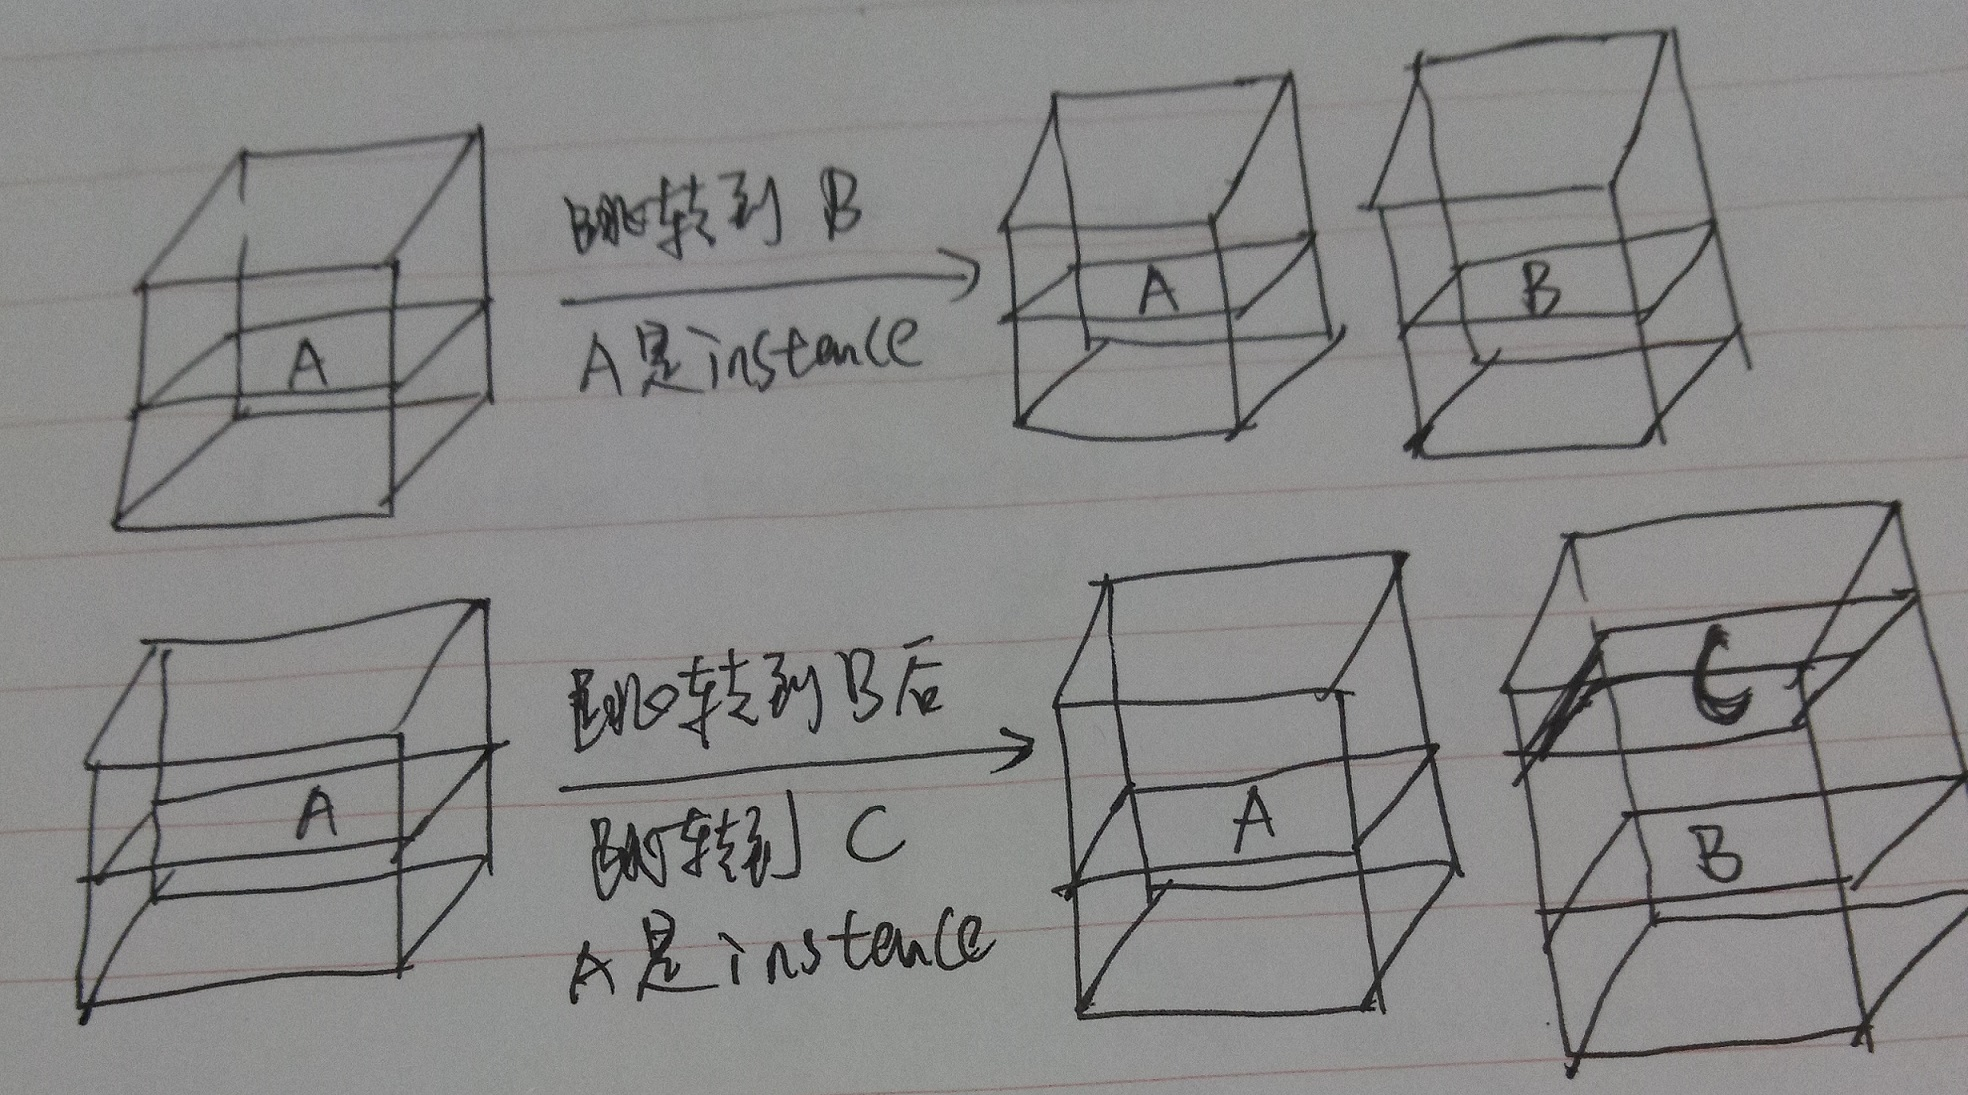
\includegraphics[width=.9\linewidth]{./pic/singleInstance.jpg}
\begin{itemize}
\item 这种模式的返回模式,出栈顺序是C-B-A,入栈顺序是A-B-C,最先出现,最后死亡
\end{itemize}

\section{综合比较与汇总}
\label{sec-4-5}

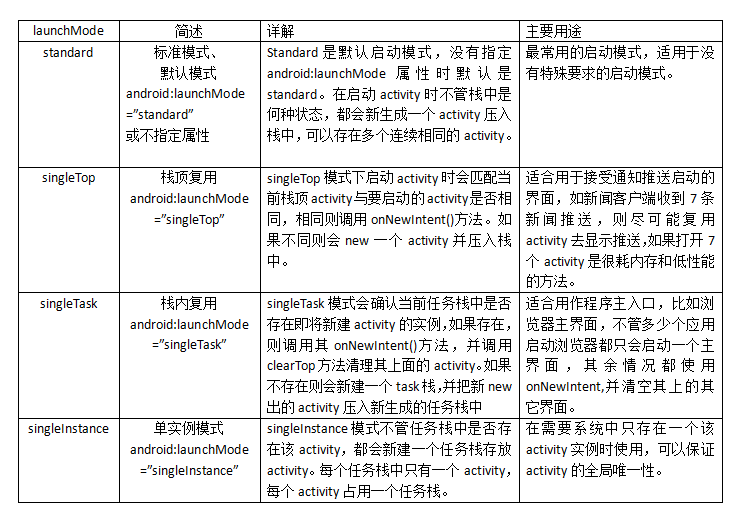
\includegraphics[width=.9\linewidth]{./pic/launchmode.png}

\section{设定方法}
\label{sec-4-6}
\begin{itemize}
\item 怎么设定这四种模式,有两种方法,
\end{itemize}
\subsection{manifest.xml文件中设置。}
\label{sec-4-6-1}
\begin{minted}[frame=lines,fontsize=\scriptsize,linenos=false]{xml}
<activity android:name=".Activity1" 
          android:launchMode="standard" 
          android:label="@string/app_name"> 
  <intent-filter> 
    <action android:name="android.intent.action.MAIN" /> 
    <category android:name="android.intent.category.LAUNCHER" /> 
  </intent-filter> 
</activity>
\end{minted}
\subsection{Intent设置标记位}
\label{sec-4-6-2}
\begin{itemize}
\item Intent设置标记位方式的优先级高于manifest中指定launchMode的方式.
\end{itemize}
\begin{enumerate}
\item FLAG$_{\text{ACTIVITY}}$$_{\text{NEW}}$$_{\text{TASK:}}$
\label{sec-4-6-2-1}
\begin{itemize}
\item 效果和在manifest中设置launchMode为singleTask相同。
\item 该标志位表示使用一个新的Task来启动一个Activity,相当于在清单文件中给Activity指定“singleTask”启动模式。通常我们在Service启动Activity时,由于Service中并没有Activity任务栈,所以必须使用该Flag来创建一个新的Task。
\end{itemize}
\item FLAG$_{\text{ACTIVITY}}$$_{\text{SINGLE}}$$_{\text{TOP:}}$
\label{sec-4-6-2-2}
\begin{itemize}
\item 这个FLAG就相当于加载模式中的singletop,比如说原来栈中情况是A,B,C,D在D中启动D,栈中的情况还是A,B,C,D
\end{itemize}
\item FLAG$_{\text{ACTIVITY}}$$_{\text{CLEAR}}$$_{\text{TOP:}}$
\label{sec-4-6-2-3}
\begin{itemize}
\item 具有此标记的activity启动时,在同一任务栈中所有位于它上面的activity都要出栈。一般和FLAG$_{\text{ACTIVITY}}$$_{\text{NEW}}$$_{\text{TASK配合使用。这种情况下,被启动的activity的实例如果已经存在,那么会调用它的onNewIntent方法。}}$
\item 这个FLAG就相当于加载模式中的SingleTask,这种FLAG启动的Activity会把要启动的Activity之上的Activity全部弹出栈空间。类如:原来栈中的情况是A,B,C,D这个时候从D中跳转到B,这个时候栈中的情况就是A,B了.
\end{itemize}
\item FLAG$_{\text{ACTIVITY}}$$_{\text{EXCLUDE}}$$_{\text{FROM}}$$_{\text{RECENTS:}}$
\label{sec-4-6-2-4}
\begin{itemize}
\item 具有此标记的activity不会出现在历史activity列表中。
\item 使用该标识位启动的Activity不添加到最近应用列表,也即我们从最近应用里面查看不到我们启动的这个activity。
\item 等同于在manifest中设置activity属性
\end{itemize}
\begin{minted}[frame=lines,fontsize=\scriptsize,linenos=false]{xml}
android:excludeFromRecents="true"
\end{minted}
\item Intent.FLAG$_{\text{ACTIVITY}}$$_{\text{NO}}$$_{\text{HISTORY}}$
\label{sec-4-6-2-5}
- 使用该模式来启动Activity,当该Activity启动其他Activity后,该Activity就被销毁了,不会保留在任务栈中。如A-B,B中以这种模式启动C,C再启动D,则任务栈只有ABD。
\item FLAG$_{\text{ACTIVITY}}$$_{\text{CLEAR}}$$_{\text{TASK}}$
\label{sec-4-6-2-6}
\begin{itemize}
\item 如果在传递给Context.startActivity()的意图中设置了该标志,则会导致在启动activity 之前清除与该activity关联的任何现有任务。也就是说,activity成为一个空任务的新根,任何旧activity都finish了。
\item 这只能与FLAG$_{\text{ACTIVITY}}$$_{\text{NEW}}$$_{\text{TASK一起使用。}}$
\end{itemize}

\item 注意事项:
\label{sec-4-6-2-7}
\begin{itemize}
\item 当通过非activity的context来启动一个activity时,需要增加intent flag FLAG$_{\text{ACTIVITY}}$$_{\text{NEW}}$$_{\text{TASK}}$
\end{itemize}
\begin{minted}[frame=lines,fontsize=\scriptsize,linenos=false]{java}
Intent i = new Intent(this, Wakeup.class);
i.addFlags(Intent.FLAG_ACTIVITY_NEW_TASK);
\end{minted}
\begin{enumerate}
\item 对 Intent.FLAG$_{\text{ACTIVITY}}$$_{\text{NEW}}$$_{\text{TASK}}$ 这个属性,是不是一定新开一个栈?
\label{sec-4-6-2-7-1}
\begin{itemize}
\item 这个问题的答案是 :不一定
\item 假设现在有一个栈1,里面是A,B,C。此时,在C中启动D的时候,设置FLAG$_{\text{ACTIVITY}}$$_{\text{NEW}}$$_{\text{TASK标记,此时会有两种情况:}}$
\begin{itemize}
\item 1.如果D这个Activity在Manifest.xml中的声明中添加了Task Affinity,系统首先会查找有没有和D的Task Affinity相同的Task栈存在,如果有存在,将D压入那个栈
\item 2.如果D这个Activity在Manifest.xml中的Task Affinity默认没有设置,则会把其压入栈1,变成:A B C D,这样就和标准模式效果是一样的了。
\end{itemize}
\item \uline{我想,这篇里的部分结论,很大一部分结论,还是需要小项目代码再验证一下其正确性的} 不敢轻信、没有确信!!!
\begin{itemize}
\item 也就是说,设置了这个标志后,新启动的Activity并非就一定在新的Task中创建,如果A和B在属于同一个package,而且都是使用默认的Task Affinity,那B还是会在A的task中被创建。 所以,只有A和B的Task Affinity不同时,设置了这个标志才会使B被创建到新的Task。
\item !注意如果试图从非Activity的非正常途径启动一个Activity,比如从一个Receiver中启动一个Activity,则Intent必须要添加FLAG$_{\text{ACTIVITY}}$$_{\text{NEW}}$$_{\text{TASK标记。}}$
\item 我们这里之所以会新建一个栈,因为我们的APP和系统Activity的Task Affinity不同
\end{itemize}
\end{itemize}
\end{enumerate}
\end{enumerate}

\subsection{Intent flag标记位进阶: (这个难度比较高一点儿,改天脑袋清醒的时候再好好理解消化一下)}
\label{sec-4-6-3}
\begin{itemize}
\item \url{https://blog.csdn.net/vshuang/article/details/66472338?spm=1001.2101.3001.6661.1&utm_medium=distribute.pc_relevant_t0.none-task-blog-2\%7Edefault\%7ECTRLIST\%7Edefault-1.no_search_link&depth_1-utm_source=distribute.pc_relevant_t0.none-task-blog-2\%7Edefault\%7ECTRLIST\%7Edefault-1.no_search_link}
\end{itemize}
\begin{enumerate}
\item FLAG$_{\text{ACTIVITY}}$$_{\text{CLEAR}}$$_{\text{TOP}}$
\label{sec-4-6-3-1}
  如果设置,并且这个Activity已经在当前的Task中运行,因此,不再是重新启动一个这个Activity的实例,而是在这个Activity上方的所有Activity都将关闭,然后这个Intent会作为一个新的Intent投递到老的Activity(现在位于顶端)中。      例如,假设一个Task中包含这些Activity:A,B,C,D。如果D调用了startActivity(),并且包含一个指向Activity B的Intent,那么,C和D都将结束,然后B接收到这个Intent,因此,目前stack的状况是:A,B。      上例中正在运行的Activity B既可以在onNewIntent()中接收到这个新的Intent,也可以把自己关闭然后重新启动来接收这个Intent。如果它的启动模式声明为“multiple”(默认值),并且你没有在这个Intent中设置FLAG$_{\text{ACTIVITY}}$$_{\text{SINGLE}}$$_{\text{TOP标志,那么它将关闭然后重新创建;对于其它的启动模式,或者在这个Intent中设置FLAG}}$$_{\text{ACTIVITY}}$$_{\text{SINGLE}}$$_{\text{TOP标志,都将把这个Intent投递到当前这个实例的onNewIntent}}$()中。      这个启动模式还可以与FLAG$_{\text{ACTIVITY}}$$_{\text{NEW}}$$_{\text{TASK结合起来使用:用于启动一个Task中的根Activity,它会把那个Task中任何运行的实例带入前台,然后清除它直到根Activity。这非常有用,例如,当从Notification}}$ Manager处启动一个Activity
\item FLAG$_{\text{ACTIVITY}}$$_{\text{CLEAR}}$$_{\text{WHEN}}$$_{\text{TASK}}$$_{\text{RESET}}$
\label{sec-4-6-3-2}
  如果设置,这将在Task的Activity stack中设置一个还原点,当Task恢复时,需要清理Activity。也就是说,下一次Task带着FLAG$_{\text{ACTIVITY}}$$_{\text{RESET}}$$_{\text{TASK}}$$_{\text{IF}}$$_{\text{NEEDED标记进入前台时(典型的操作是用户在主画面重启它),这个Activity和它之上的都将关闭,以至于用户不能再返回到它们,但是可以回到之前的Activity。}}$      这在你的程序有分割点的时候很有用。例如,一个e-mail应用程序可能有一个操作是查看一个附件,需要启动图片浏览Activity来显示。这个Activity应该作为e-mail应用程序Task的一部分,因为这是用户在这个Task中触发的操作。然而,当用户离开这个Task,然后从主画面选择e-mail app,我们可能希望回到查看的会话中,但不是查看图片附件,因为这让人困惑。通过在启动图片浏览时设定这个标志,浏览及其它启动的Activity在下次用户返回到mail程序时都将全部清除。
\item FLAG$_{\text{ACTIVITY}}$$_{\text{RESET}}$$_{\text{TASK}}$$_{\text{IF}}$$_{\text{NEEDED}}$
\label{sec-4-6-3-3}
  If set, and this activity is either being started in a new task or bringing to the top an existing task, then it will be launched as the front door of the task. This will result in the application of any affinities needed to have that task in the proper state (either moving activities to or from it), or simply resetting that task to its initial state if needed.
\item FLAG$_{\text{ACTIVITY}}$$_{\text{NEW}}$$_{\text{TASK}}$
\label{sec-4-6-3-4}
   如果设置,这个Activity会成为历史stack中一个新Task的开始。一个Task(从启动它的Activity到下一个Task中的Activity)定义了用户可以迁移的Activity原子组。Task可以移动到前台和后台;在某个特定Task中的所有Activity总是保持相同的次序。      这个标志一般用于呈现“启动”类型的行为:它们提供用户一系列可以单独完成的事情,与启动它们的Activity完全无关。      使用这个标志,如果正在启动的Activity的Task已经在运行的话,那么,新的Activity将不会启动;代替的,当前Task会简单的移入前台。参考FLAG$_{\text{ACTIVITY}}$$_{\text{MULTIPLE}}$$_{\text{TASK标志,可以禁用这一行为。}}$      这个标志不能用于调用方对已经启动的Activity请求结果。
\item FLAG$_{\text{ACTIVITY}}$$_{\text{EXCLUDE}}$$_{\text{FROM}}$$_{\text{RECENTS}}$
\label{sec-4-6-3-5}
\begin{itemize}
\item 如果设置,新的Activity不会在最近启动的Activity的列表中保存。
\item 参考一个stackoverflow的问答 \url{https://stackoverflow.com/questions/7759556/flag-activity-exclude-from-recents-excludes-whole-application-not-only-the-acti}
\item I have a Notification which starts an Activity. After a long press on home button and selecting my app, I want to start my main Activity again, and not this Activity started by the Notification. I tried with FLAG$_{\text{ACTIVITY}}$$_{\text{EXCLUDE}}$$_{\text{FROM}}$$_{\text{RECENTS}}$, but this removed my whole application from the recents, and that's not what I want to achieve. How can I have my app in the recents, but have the main Activity started?
\item Okay, I found the solution to my problem. I started an Activity from a Notification with FLAG$_{\text{ACTIVITY}}$$_{\text{NEW}}$$_{\text{TASK}}$. But it seems to me that this Activity only gets started in an own task if affinity is different from the default affinity. So I had to add a different affinity in the manifest.
\item And it seems that FLAG$_{\text{ACTIVITY}}$$_{\text{EXCLUDE}}$$_{\text{FROM}}$$_{\text{RECENTS}}$ does not (as documented) exlucde the Activity from the recents, rather it excludes the whole task (not the whole application) in which the Activity gets started from the recents. And as I hadn't set a different affinity the Activity which I wanted to exclude was started in the same task (although I had set FLAG$_{\text{ACTIVITY}}$$_{\text{NEW}}$$_{\text{TASK}}$) and so my whole application (as it was running in only one task) was excluded from the recents.
\item Now I've set a different affinity for the Activity that gets started from the Notification and I start it with FLAG$_{\text{ACTIVITY}}$$_{\text{NEW}}$$_{\text{TASK}}$ | FLAG$_{\text{ACTIVITY}}$$_{\text{EXCLUDE}}$$_{\text{FROM}}$$_{\text{RECENTS}}$. When I leave this Activity and long-press the HOME button I can choose my app and the default task is started or brought to the front.
\end{itemize}
\item FLAG$_{\text{ACTIVITY}}$$_{\text{FORWARD}}$$_{\text{RESULT}}$
\label{sec-4-6-3-6}
\begin{itemize}
\item 如果设置,并且这个Intent用于从一个存在的Activity启动一个新的Activity,那么,这个作为答复目标的Activity将会传到这个新的Activity中。这种方式下,新的Activity可以调用setResult(int),并且这个结果值将发送给那个作为答复目标的Activity。
\end{itemize}
\end{enumerate}

\section{启动模式与startActivityForResult}
\label{sec-4-7}
\subsection{LaunchMode与StartActivityForResult}
\label{sec-4-7-1}
\begin{itemize}
\item 我们在开发过程中经常会用到StartActivityForResult方法启动一个Activity,然后在onActivityResult()方法中可以接收到上个页面的回传值,但你有可能遇到过拿不到返回值的情况,那有可能是因为Activity的LaunchMode设置为了singleTask。5.0之后,android的LaunchMode与StartActivityForResult的关系发生了一些改变。两个Activity,A和B,现在由A页面跳转到B页面,看一下LaunchMode与StartActivityForResult之间的关系:
\item 这是为什么呢?
\item 这是因为ActivityStackSupervisor类中的startActivityUncheckedLocked方法在5.0中进行了修改。
\item 在5.0之前,当启动一个Activity时,系统将首先检查Activity的launchMode,如果为A页面设置为SingleInstance或者B页面设置为singleTask或者singleInstance,则会在LaunchFlags中加入FLAG$_{\text{ACTIVITY}}$$_{\text{NEW}}$$_{\text{TASK标志,而如果含有FLAG}}$$_{\text{ACTIVITY}}$$_{\text{NEW}}$$_{\text{TASK标志的话,onActivityResult将会立即接收到一个cancle的信息。}}$
\end{itemize}
\begin{minted}[frame=lines,fontsize=\scriptsize,linenos=false]{java}
final boolean launchSingleTop = r.launchMode == ActivityInfo.LAUNCH_SINGLE_TOP;
final boolean launchSingleInstance = r.launchMode == ActivityInfo.LAUNCH_SINGLE_INSTANCE;
final boolean launchSingleTask = r.launchMode == ActivityInfo.LAUNCH_SINGLE_TASK;
int launchFlags = intent.getFlags();
if ((launchFlags & Intent.FLAG_ACTIVITY_NEW_DOCUMENT) != 0 &&
        (launchSingleInstance || launchSingleTask)) {
    // We have a conflict between the Intent and the Activity manifest, manifest wins.
    Slog.i(TAG, "Ignoring FLAG_ACTIVITY_NEW_DOCUMENT, launchMode is " +
            "\"singleInstance\" or \"singleTask\"");
    launchFlags &=
            ~(Intent.FLAG_ACTIVITY_NEW_DOCUMENT | Intent.FLAG_ACTIVITY_MULTIPLE_TASK);
} else {
    switch (r.info.documentLaunchMode) {
        case ActivityInfo.DOCUMENT_LAUNCH_NONE:
            break;
        case ActivityInfo.DOCUMENT_LAUNCH_INTO_EXISTING:
            launchFlags |= Intent.FLAG_ACTIVITY_NEW_DOCUMENT;
            break;
        case ActivityInfo.DOCUMENT_LAUNCH_ALWAYS:
            launchFlags |= Intent.FLAG_ACTIVITY_NEW_DOCUMENT;
            break;
        case ActivityInfo.DOCUMENT_LAUNCH_NEVER:
            launchFlags &= ~Intent.FLAG_ACTIVITY_MULTIPLE_TASK;
            break;
    }
}
final boolean launchTaskBehind = r.mLaunchTaskBehind
        && !launchSingleTask && !launchSingleInstance
        && (launchFlags & Intent.FLAG_ACTIVITY_NEW_DOCUMENT) != 0;
if (r.resultTo != null && (launchFlags & Intent.FLAG_ACTIVITY_NEW_TASK) != 0) {
    // For whatever reason this activity is being launched into a new
    // task...  yet the caller has requested a result back.  Well, that
    // is pretty messed up, so instead immediately send back a cancel
    // and let the new task continue launched as normal without a
    // dependency on its originator.
    Slog.w(TAG, "Activity is launching as a new task, so cancelling activity result.");
    r.resultTo.task.stack.sendActivityResultLocked(-1,
            r.resultTo, r.resultWho, r.requestCode,
            Activity.RESULT_CANCELED, null);
    r.resultTo = null;
}
\end{minted}
\begin{itemize}
\item 而5.0之后这个方法做了修改,修改之后即便启动的页面设置launchMode为singleTask或singleInstance,onActivityResult依旧可以正常工作,也就是说无论设置哪种启动方式,StartActivityForResult和onActivityResult()这一组合都是有效的。所以如果你目前正好基于5.0做相关开发,不要忘了向下兼容,这里有个坑请注意避让。
\item \uline{所以下面的结论可能不对,需要改天代码再好好验证一下}
\begin{minted}[frame=lines,fontsize=\scriptsize,linenos=false]{java}
if (sourceRecord == null) {
    // This activity is not being started from another...  
    // in this case we -ALWAYS- start a new task.
    if ((launchFlags & Intent.FLAG_ACTIVITY_NEW_TASK) == 0) {
        Slog.w(TAG, "startActivity called from non-Activity context; forcing Intent.FLAG_ACTIVITY_NEW_TASK for: "
              + intent);
        launchFlags |= Intent.FLAG_ACTIVITY_NEW_TASK;
    }
} else if (sourceRecord.launchMode == ActivityInfo.LAUNCH_SINGLE_INSTANCE) {
    // The original activity who is starting us is running as a single
    // instance...  this new activity it is starting must go on its
    // own task.
    launchFlags |= Intent.FLAG_ACTIVITY_NEW_TASK;
} else if (r.launchMode == ActivityInfo.LAUNCH_SINGLE_INSTANCE
        || r.launchMode == ActivityInfo.LAUNCH_SINGLE_TASK) {
    // The activity being started is a single instance...  it always
    // gets launched into its own task.
    launchFlags |= Intent.FLAG_ACTIVITY_NEW_TASK;
}
if (r.resultTo != null && (launchFlags&Intent.FLAG_ACTIVITY_NEW_TASK) != 0) {
    // For whatever reason this activity is being launched into a new
    // task...  yet the caller has requested a result back.  Well, that
    // is pretty messed up, so instead immediately send back a cancel
    // and let the new task continue launched as normal without a
    // dependency on its originator.
    Slog.w(TAG, "Activity is launching as a new task, so cancelling activity result.");
    sendActivityResultLocked(-1,
            r.resultTo, r.resultWho, r.requestCode,
        Activity.RESULT_CANCELED, null);
    r.resultTo = null;
}
\end{minted}
\item 也就是说startActivityForResult启动的activity有FLAG$_{\text{ACTIVITY}}$$_{\text{NEW}}$$_{\text{TASK,那么就不能返回结果。}}$( \uline{这个结论可能太古老了吧?!!!} )
\end{itemize}
\subsection{启动任务(Task): 这里要再消化一下!}
\label{sec-4-7-2}
\begin{itemize}
\item Intent filter中有”android.intent.action.MAIN ” action和”android.intent.category.LAUNCHER ” category的activity将被标记为task的入口。带有这两个标记的activity将会显示在应用程序启动器(application launcher)中。
\item 第二个比较重要的点是, \uline{用户必须能够离开task并在之后返回} 。因为这个原因,singleTask和singleInstance这两种运行模式只能应用于含有MAIN和LAUNCHER过滤器的 activity 。打个比方,如果不包含带MAIN和LAUNCHER过滤器,某个activity运行了一个singleTask模式的 activity,初始化了一个新的task,当用户按下HOME键时,那个activity就被主屏幕“挡住”了,用户再也无法返回到那个 activity。 (这里读得昏昏乎乎!!!)
\item 类似的情况在FLAG$_{\text{ACTIVITY}}$$_{\text{NEW}}$$_{\text{TASK标记上也会出现。如果这个标记会新建一个task,当用户按下HOME键时,必须有一种}}$ 方式能够让用户返回到那个activity。有些东西(比如notification manager)总是要求在外部task中启动activity,在传递给startActivity的intent中总是包含 FLAG$_{\text{ACTIVITY}}$$_{\text{NEW}}$$_{\text{TASK标记。}}$
\item 对于那种不希望用户离开之后再返回activity的情况,可将finishOnTaskLaunch属性设置为true。
\end{itemize}
\subsection{Activity Stack}
\label{sec-4-7-3}
\begin{itemize}
\item 可以通过 adb shell dumpsys | grep ActivityRecord 来查看 TASKS的ActivityStacks
\item 可以通过 adb shell dumpsys activity activities | grep packageName| grep Run 来查看某个packageName的ActivityStatcks
\end{itemize}

\section{onNewIntent}
\label{sec-4-8}
\begin{itemize}
\item 当通过singleTop/singleTask启动activity时,如果满足复用条件,则不会创建新的activity实例,生命周期就变为onNewIntent()---->onResart()------>onStart()----->onResume()。
\begin{itemize}
\item Activity第一启动的时候执行onCreate()---->onStart()---->onResume()等后续生命周期函数,也就时说第一次启动Activity并不会执行到onNewIntent().;
\item 而后面如果再有想启动Activity的时候,那就是执行onNewIntent()---->onResart()------>onStart()----->onResume();
\item 如果android系统由于内存不足把已存在Activity释放掉了,那么再次调用的时候会重新启动Activity即执行onCreate()---->onStart()---->onResume()等。
\end{itemize}
\item 注意:当调用到onNewIntent(intent)的时候,需要在onNewIntent() 中使用setIntent(intent)赋值给Activity的Intent.否则,后续的getIntent()都是得到老的Intent。
\end{itemize}

\section{Activity所需的任务栈与TaskAffinity}
\label{sec-4-9}
\begin{itemize}
\item 这要从一个参数说起:TaskAffinity(任务相关性)。这个参数标识了一个activity所需的任务栈的名字,默认情况下,所有activity所需的任务栈的名字为应用的包名。
\item TaskAffinity 参数标识着Activity所需要的任务栈的名称,默认情况下,一个应用中所有Activity所需要的任务栈名称都为该应用的包名。
\item TaskAffinity 属性一般跟singleTask模式或者跟allowTaskReparenting属性结合使用,在其他情况下没有实际意义。
\end{itemize}
\subsection{TaskAffinity和singleTask启动模式结合使用}
\label{sec-4-9-1}
\begin{itemize}
\item 当TaskAffinity和singleTask启动模式结合使用时,当前Activity的任务栈名称将与TaskAffinity属性指定的值相同,下面我们通过代码来验证,我们同过MainActivity来启动ActivityA,其中MainActivity启动模式为默认模式,ActivityA启动模式为singleTask,而TaskAffinity属性值为android:taskAffinity="com.zejian.singleTask.affinity"
\end{itemize}
\begin{minted}[frame=lines,fontsize=\scriptsize,linenos=false]{xml}
<?xml version="1.0" encoding="utf-8"?>
<manifest xmlns:android="http://schemas.android.com/apk/res/android"
          package="comzejian.myapplication">
  <application
      android:allowBackup="true"
      android:icon="@mipmap/ic_launcher"
      android:label="@string/app_name"
      android:supportsRtl="true"
      android:theme="@style/AppTheme">

    <activity android:name=".MainActivity">
      <intent-filter>
        <action android:name="android.intent.action.MAIN" />
        <category android:name="android.intent.category.LAUNCHER" />
      </intent-filter>
    </activity>

    <activity android:name=".ActivityA"
              android:launchMode="singleTask"
              android:taskAffinity="com.zejian.singleTask.affinity"
              />
    
  </application>
</manifest>
\end{minted}
\begin{itemize}
\item 可以通过singleTask与android:taskAffinity属性相结合的方式来指定我们Activity所需要的栈名称,使相应的Activity存在于不同的栈中
\end{itemize}
\subsection{当TaskAffinity和allowTaskReparenting结合使用}
\label{sec-4-9-2}
\begin{enumerate}
\item allowTaskReparenting属性
\label{sec-4-9-2-1}
\begin{itemize}
\item 它的主要作用是activity的迁移,即从一个task迁移到另一个task,这个迁移跟activity的taskAffinity有关。
\begin{itemize}
\item 当allowTaskReparenting的值为“true”时,则表示Activity能从启动的Task移动到有着affinity的Task(当这个Task进入到前台时),
\item 当allowTaskReparenting的值为“false”,表示它必须呆在启动时呆在的那个Task里。如果这个特性没有被设定,元素(当然也可以作用在每次activity元素上)上的allowTaskReparenting属性的值会应用到Activity上。默认值为“false”。
\end{itemize}
\end{itemize}

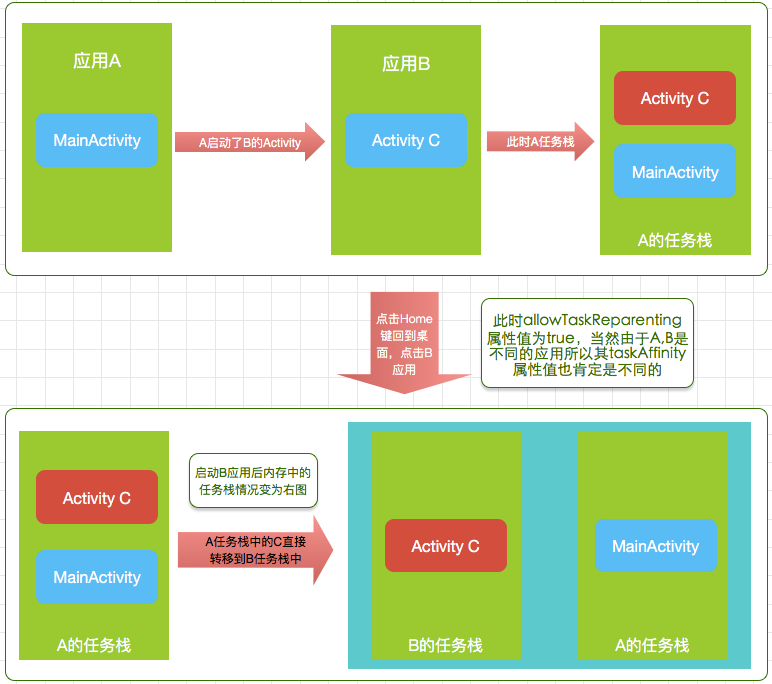
\includegraphics[width=.9\linewidth]{./pic/reparenting.png}

\begin{itemize}
\item 举个例子,比如现在有两个应用A和B,A启动了B的一个ActivityC,然后按Home键回到桌面,再单击B应用时,如果此时,allowTaskReparenting的值为“true”,那么这个时候并不会启动B的主Activity,而是直接显示已被应用A启动的ActivityC,我们也可以认为ActivityC从A的任务栈转移到了B的任务栈中。
\end{itemize}
\begin{enumerate}
\item 用代码来码证一下
\label{sec-4-9-2-1-1}
\begin{itemize}
\item ActivityA
\end{itemize}
\begin{minted}[frame=lines,fontsize=\scriptsize,linenos=false]{java}
public class ActivityA extends Activity {
    private Button btnC;
    @Override
        protected void onCreate(Bundle savedInstanceState) {
        super.onCreate(savedInstanceState);
        setContentView(R.layout.activity_a);
        btnC = (Button) findViewById(R.id.mainC);
        btnC.setOnClickListener(new View.OnClickListener() {
                @Override public void onClick(View v) {
                    Intent intent = new Intent(Intent.ACTION_MAIN);
                    intent.addCategory(Intent.CATEGORY_LAUNCHER); // 去打开B应用中的activity 
                    ComponentName cn = new ComponentName("com.cmcm.activitytask2", "com.cmcm.activitytask2.ActivityC");
                    intent.setComponent(cn);
                    startActivity(intent);
                }
            });
    }
}
\end{minted}
\begin{itemize}
\item A 应用的 manifest.xml
\end{itemize}
\begin{minted}[frame=lines,fontsize=\scriptsize,linenos=false]{xml}
<activity android:name=".ActivityA">
     <intent-filter>
           <action android:name="android.intent.action.MAIN" />
           <category android:name="android.intent.category.LAUNCHER" />
     </intent-filter>
</activity>
\end{minted}
\begin{itemize}
\item B应用中的启动模式以及标志位的设置
\end{itemize}
\begin{minted}[frame=lines,fontsize=\scriptsize,linenos=false]{java}
public class ActivityC extends Activity {
    @Override
    protected void onCreate(Bundle savedInstanceState) {
        super.onCreate(savedInstanceState);
        setContentView(R.layout.activity_c);
    }
}
\end{minted}
\begin{itemize}
\item B应用的manifest.xml
\end{itemize}
\begin{minted}[frame=lines,fontsize=\scriptsize,linenos=false]{xml}
<activity android:name=".ActivityC" android:exported="true"    
      android:allowTaskReparenting="true">
</activity>
\end{minted}
\item 查看Activity的返回栈
\label{sec-4-9-2-1-2}
\begin{itemize}
\item adb shell dumpsys activity // 找
\item ACTIVITY MANAGER RECENT TASKS (dumpsys activity recents)
\item ACTIVITY MANAGER ACTIVITIES (dumpsys activity activities)
\end{itemize}
\end{enumerate}
\item 注意点
\label{sec-4-9-2-2}
\begin{itemize}
\item 有点需要说明的是allowTaskReparenting仅限于singleTop和standard模式,这是因为一个activity的affinity属性由它的taskAffinity属性定义(代表栈名),而一个task的affinity由它的root activity定义。所以,一个task的root activity总是拥有和它所在task相同的affinity。
\item 由于以singleTask和singleInstance启动的activity只能是一个task的root activity,因此allowTaskReparenting仅限于以standard 和singleTop启动的activity
\item 列一下清单文件中 <activity>元素的几个关键属性
\begin{itemize}
\item launchMode
\item taskAffinity
\item allowTaskReparenting
\item clearTaskOnLaunch
\item alwaysRetainTaskState
\item finishOnTaskLaunch
\end{itemize}
\end{itemize}
\item taskAffinity在两种情况下起作用:
\label{sec-4-9-2-3}
\begin{enumerate}
\item 当启动Activity的Intent中带有FLAG$_{\text{ACTIVITY}}$$_{\text{NEW}}$$_{\text{TASK标志时。}}$
\label{sec-4-9-2-3-1}
\begin{itemize}
\item 在默认情况下,目标Activity将与startActivity的调用者处于同一task中。但如果用户特别指定了FLAG$_{\text{ACTIVITY}}$$_{\text{NEW}}$$_{\text{TASK,表明它希望为Activity重新开设一个Task。这时就有两种情况:}}$
\begin{itemize}
\item 假如当前已经有一个Task,它的affinity与新Activity是一样的,那么系统会直接用此Task来完成操作,而不是另外创建一个Task;
\item 否则系统需要创建一个Task。
\end{itemize}
\end{itemize}
\item 当Activity中的allowTaskReparenting属性设置为true时。
\label{sec-4-9-2-3-2}
\begin{itemize}
\item 在这种情况下,Activity具有"动态转移"的能力。举个前面的"短信"例子,在默认情况下,该应用程序中的所有Activity具有相同的affinity。
\item 当另一个程序启动了"短信编辑"时,一开始这个Activity和启动它的Activity处于同样的Task中。但如果"短信编辑"Activity指定了allowTaskReparenting,且后期"短信"程序的Task转为前台,此时"短信编辑"这一Activity会被"挪"到与它更亲近的"短信"Task中。
\end{itemize}
\end{enumerate}
\end{enumerate}

\subsection{清空任务栈}
\label{sec-4-9-3}
\begin{itemize}
\item Android系统除了给我提供了TaskAffinity来指定任务栈名称外,还给我提供了清空任务栈的方法,在一般情况下我们只需要在<activity>标签中指明相应的属性值即可。
\end{itemize}
\begin{enumerate}
\item clearTaskOnLaunch
\label{sec-4-9-3-1}
\begin{minted}[frame=lines,fontsize=\scriptsize,linenos=false]{xml}
android:clearTaskOnLaunch
\end{minted}
\begin{itemize}
\item 这个属性用来标记是否从task清除除根Activity之外的所有的Activity,“true”表示清除,“false”表示不清除,默认为“false”。这里有点我们必须要注意的,这个属性只对任务栈内的root Activity起作用,任务栈内其他的Activity都会被忽略。如果android:clearTaskOnLaunch属性为“true”,每次我们重新进入这个应用时,我们只会看到根Activity,任务栈中的其他Activity都会被清除出栈。
\item 比如一个应用的Activity A,B,C,其中clearTaskOnLaunch设置为true,C为默认值,我们依次启动A,B,C,点击HOME,再在桌面点击图标。启动的是A,而B,C将都被移除当前任务栈。也就是说,当Activity的属性clearTaskOnLaunch为true时将被优先启动,其余的Activity(B、C)都被移除任务栈并销毁,除非前面A已经finish销毁,后面的已注册clearTaskOnLaunch为true的activity(B)才会生效。
\end{itemize}
- 特别地,如果我们的应用中引用到了其他应用的Activity,这些Activity设置了android:allowTaskReparenting属性为“true”,则它们会被重新宿主到有共同affinity的task中。
\item android:finishOnTaskLaunch
\label{sec-4-9-3-2}
- finishOnTaskLaunch属性与clearTaskOnLaunch 有些类似,它们的区别是finishOnTaskLaunch是作用在自己身上(把自己移除任务栈,不影响别的Activity),而clearTaskOnLaunch则是作用在别人身上(把别的Activity移除任务栈),如果我们把Activity的android:finishOnTaskLaunch属性值设置为true时,离开这个Activity所依赖的任务栈后,当我们重新返回时,该Activity将会被finish掉,而且其他Activity不会受到影响。
\item android:alwaysRetainTaskState
\label{sec-4-9-3-3}
- alwaysRetainTaskState实际上是给了当前Activity所在的任务栈一个“免死金牌”,如果当前Activity的android:alwaysRetainTaskState设置为true时,那么该Activity所在的任务栈将不会受到任何清理命令的影响,一直保持当前任务栈的状态。
\end{enumerate}

\section{启动模式的应用场景}
\label{sec-4-10}
\subsection{SingleTask模式的运用场景}
\label{sec-4-10-1}
\begin{itemize}
\item 最常见的应用场景就是保持我们应用开启后仅仅有一个Activity的实例。最典型的样例就是应用中展示的主页(Home页)。
\item 假设用户在主页跳转到其他页面,运行多次操作后想返回到主页,假设不使用SingleTask模式,在点击返回的过程中会多次看到主页,这明显就是设计不合理了。
\end{itemize}
\subsection{SingleTop模式的运用场景}
\label{sec-4-10-2}
\begin{itemize}
\item 假设你在当前的Activity中又要启动同类型的Activity,此时建议将此类型Activity的启动模式指定为SingleTop,能够降低Activity的创建,节省内存!
\end{itemize}
\subsection{SingleInstance模式的运用场景}
\label{sec-4-10-3}
\begin{itemize}
\item SingleInstance是activity启动的一种模式,一般做应用层开发很少用到,我一般用到的app定时提醒会用到这个模式吧。这个模式使用起来有很多坑,假设有activityA,activityB,activityC这三个activity,我们将activityB设置为SingleInstance
\end{itemize}
\begin{enumerate}
\item 第一种情况
\label{sec-4-10-3-1}
\begin{itemize}
\item A开启B,B开启C,如果finish activityC,那么activityA会显示而不是我们想要的activityB,这是因为activityB和activityA、activityC所处的栈不同,C关闭了,就要显示C所处栈的下一个activity,解决这个问题办法很多,我自己用的方法是通过记录开启activity,在被关闭的activity的finish方法中重新开启activityB。
\end{itemize}
\item 第二种情况
\label{sec-4-10-3-2}
A开启B,然后按home键,再从左面点开应用,显示的是A,这是因为launch启动我们应用的时候 会从默认的栈找到栈顶的activity显示,这个解决办法的思路跟第一种差不多,也就不献丑了
\item 第三种情况
\label{sec-4-10-3-3}
\begin{itemize}
\item A开启C,C开启B,B开启A,结果显示的是C,这还是两个栈造成的,B开启A的时候,其实是到达A所处的栈,栈顶是C,所以就显示C了,解决办法是用flag把默认栈activity清理了,重新开启A,或者回退到C时再开启A。
\end{itemize}
\item 总结
\label{sec-4-10-3-4}
\begin{itemize}
\item 三种情况的解决方法都是基于页面少的情况,如果页面多了会产生更多的问题
\item 为了必避免这个问题,最好不用在中间层使用SingleInstance
\item TIPS:  
\begin{itemize}
\item (1)如果想让C和B同一个栈,那就使用taskinfinity,给他俩设置同样的栈名
\item (2)onActivityResult不能与SingleInstance不能一起使用,因为不同栈
\end{itemize}
\end{itemize}
\end{enumerate}
\subsection{standard 运用场景}
\label{sec-4-10-4}
\begin{itemize}
\item Activity 的启动默认就是这种模式。在 standard 模式下,每次启动一个 Activity 都会创建一个新的实例;
\item 在正常应用中正常打开和关闭页面就可以了,退出整个app就关闭所有的页面
\end{itemize}
\section{Activity时的生命周期不同}
\label{sec-4-11}
\begin{itemize}
\item 由于当一个Activity设置了SingleTop或者SingleTask模式或者SingleInstance模式后,跳转此Activity出现复用原有Activity的情况时,此Activity的onCreate方法将不会再次运行。onCreate方法仅仅会在第一次创建Activity时被运行。
\item 而一般onCreate方法中会进行该页面的数据初始化、UI初始化,假设页面的展示数据无关页面跳转传递的參数,则不必操心此问题,若页面展示的数据就是通过getInten() 方法来获取,那么问题就会出现:getInten()获取的一直都是老数据,根本无法接收跳转时传送的新数据!
\item 这时我们须要另外一个回调 onNewIntent(Intent intent)方法。此方法会传入最新的intent,这样我们就能够解决上述问题。这里建议的方法是又一次去setIntent。然后又一次去初始化数据和UI
\end{itemize}
\begin{minted}[frame=lines,fontsize=\scriptsize,linenos=false]{java}
/** 复用Activity时的生命周期回调*/
@Override     
protected void onNewIntent(Intent intent) {         
    super.onNewIntent(intent);         
    setIntent(intent);         
    initData();         
    initView();     
}
\end{minted}
\section{实际中的栈管理类}
\label{sec-4-12}
\begin{itemize}
\item 管理Activity的类,一般在BaseActivity会调用这个类,然后所有的Activity继承BaseActivity,这样管理好整个项目的Activity
\end{itemize}
\begin{minted}[frame=lines,fontsize=\scriptsize,linenos=false]{java}
public class ActivityStackManager { // activity堆栈管理 
    private static ActivityStackManager mInstance; 
    private static Stack<Activity> mActivityStack; 
    public static ActivityStackManager getInstance() { 
        if (null == mInstance) 
            mInstance = new ActivityStackManager(); 
        return mInstance; 
    } 
    private ActivityStackManager() { 
        mActivityStack = new Stack<Activity>(); 
    } 
    public void addActivity(Activity activity) {  // 入栈 
        mActivityStack.push(activity); 
    } 
    public void removeActivity(Activity activity) {  // 出栈 
        mActivityStack.remove(activity); 
    } 
    public void finishAllActivity() {  // 彻底退出 
        Activity activity; 
        while (!mActivityStack.empty()) { 
            activity = mActivityStack.pop(); 
            if (activity != null) 
                activity.finish(); 
        } 
    } 
    public void finishActivity(Class<?> cls) {  // 结束指定类名的Activity 
        for (Activity activity : mActivityStack) { 
            if (activity.getClass().equals(cls)) { 
                finishActivity(activity); 
            } 
        } 
    } 
    public boolean checkActivity(Class<?> cls) {  // 查找栈中是否存在指定的activity 
        for (Activity activity : mActivityStack) { 
            if (activity.getClass().equals(cls)) { 
                return true; 
            } 
        } 
        return false; 
    } 
    public void finishActivity(Activity activity) {  // 结束指定的Activity 
        if (activity != null) { 
            mActivityStack.remove(activity); 
            activity.finish(); 
            activity = null; 
        } 
    } 
    public boolean finishToActivity(Class<? extends Activity> actCls, boolean isIncludeSelf) { // finish指定的activity之上所有的activity 
        List<Activity> buf = new ArrayList<Activity>(); 
        int size = mActivityStack.size(); 
        Activity activity = null; 
        for (int i = size - 1; i >= 0; i--) { 
            activity = mActivityStack.get(i); 
            if (activity.getClass().isAssignableFrom(actCls)) { 
                for (Activity a : buf) 
                    a.finish(); 
                return true; 
            } else if (i == size - 1 && isIncludeSelf) 
                buf.add(activity); 
            else if (i != size - 1) 
                buf.add(activity); 
        } 
        return false; 
    }
}
\end{minted}


\chapter{Content Provider 内存承载器}
\label{sec-5}
\begin{itemize}
\item ContentProvider的底层是采用 Android中的Binder机制
\end{itemize}
\section{统一资源标识符(URI)}
\label{sec-5-1}
\begin{itemize}
\item 定义:Uniform Resource Identifier,即统一资源标识符
\item 作用:唯一标识 ContentProvider \& 其中的数据
\begin{itemize}
\item 外界进程通过 URI 找到对应的ContentProvider \& 其中的数据,再进行数据操作
\end{itemize}
\item 具体使用
\begin{itemize}
\item URI分为 系统预置 \& 自定义,分别对应系统内置的数据(如通讯录、日程表等等)和自定义数据库
\begin{itemize}
\item 关于 系统预置URI 此处不作过多讲解,需要的同学可自行查看
\item 此处主要讲解 自定义URI
\end{itemize}
\end{itemize}
\end{itemize}

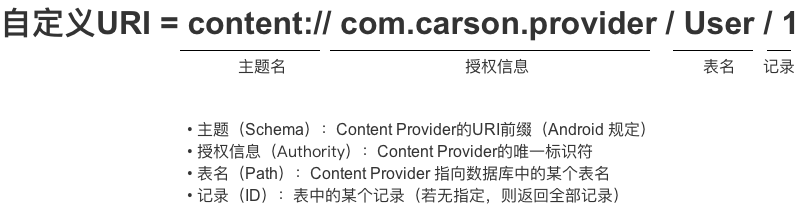
\includegraphics[width=.9\linewidth]{./pic/uri.png}

\begin{itemize}
\item 授权信息(Authority):ContentProvider的唯一标识符。所以这个一定得match对了
\end{itemize}
\begin{minted}[frame=lines,fontsize=\scriptsize,linenos=false]{java}
Uri uri = Uri.parse("content://com.carson.provider/User/1") // 设置URI
// 上述URI指向的资源是:名为 `com.carson.provider`的`ContentProvider` 中表名 为`User` 中的 `id`为1的数据

// 特别注意:URI模式存在匹配通配符: * # (两个)
//  *:匹配任意长度的任何有效字符的字符串
//     以下的URI 表示 匹配provider的任何内容
//     content://com.example.app.provider/* 
// #:匹配任意长度的数字字符的字符串
//     以下的URI 表示 匹配provider中的table表的所有行
//     content://com.example.app.provider/table/#
\end{minted}
\begin{itemize}
\item uri 的各个部分在安卓中都是可以通过代码获取的,下面我们就以下面这个 uri 为例来说下获取各个部分的方法:
\item \url{http://www.baidu.com:8080/wenku/jiatiao.html?id=123456&name=jack}
\end{itemize}
\begin{minted}[frame=lines,fontsize=\scriptsize,linenos=false]{java}
getScheme() // 获取 Uri 中的 scheme 字符串部分,在这里是 http
getHost()   // 获取 Authority 中的 Host 字符串,即 www.baidu.com
getPost()   // 获取 Authority 中的 Port 字符串,即 8080
getPath()   // 获取 Uri 中 path 部分,即 wenku/jiatiao.html
getQuery()  // 获取 Uri 中的 query 部分,即 id=15&name=du
\end{minted}

\section{MIME数据类型}
\label{sec-5-2}
\begin{itemize}
\item 作用:指定某个扩展名的文件用某种应用程序来打开
\begin{itemize}
\item 如指定.html文件采用text应用程序打开、指定.pdf文件采用flash应用程序打开
\end{itemize}
\end{itemize}

\subsection{ContentProvider根据 URI 返回MIME类型}
\label{sec-5-2-1}
\begin{minted}[frame=lines,fontsize=\scriptsize,linenos=false]{java}
ContentProvider.geType(uri) ;
\end{minted}
\subsection{MIME类型组成}
\label{sec-5-2-2}
\begin{itemize}
\item 每种MIME类型 由2部分组成 = 类型 + 子类型
\item MIME类型是 一个 包含2部分的字符串
\end{itemize}
\begin{minted}[frame=lines,fontsize=\scriptsize,linenos=false]{xml}
text / html
// 类型 = text、子类型 = html
text/css
text/xml
application/pdf
\end{minted}

\subsection{MIME类型形式}
\label{sec-5-2-3}
\begin{itemize}
\item MIME类型有2种形式:单条记录, 或是多条记录
\begin{minted}[frame=lines,fontsize=\scriptsize,linenos=false]{java}
// 形式1:单条记录  
vnd.android.cursor.item/自定义
// 形式2:多条记录(集合)
vnd.android.cursor.dir/自定义 

// 注:
  // 1. vnd:表示父类型和子类型具有非标准的、特定的形式。
  // 2. 父类型已固定好(即不能更改),只能区别是单条还是多条记录
  // 3. 子类型可自定义
\end{minted}
\item 实例说明
\end{itemize}
\begin{minted}[frame=lines,fontsize=\scriptsize,linenos=false]{xml}
<-- 单条记录 -->
  // 单个记录的MIME类型
  vnd.android.cursor.item/vnd.yourcompanyname.contenttype 

  // 若一个Uri如下
  content://com.example.transportationprovider/trains/122   
  // 则ContentProvider会通过ContentProvider.geType(url)返回以下MIME类型
  vnd.android.cursor.item/vnd.example.rail

<-- 多条记录 -->
  // 多个记录的MIME类型
  vnd.android.cursor.dir/vnd.yourcompanyname.contenttype 
  // 若一个Uri如下
  content://com.example.transportationprovider/trains 
  // 则ContentProvider会通过ContentProvider.geType(url)返回以下MIME类型
  vnd.android.cursor.dir/vnd.example.rail
\end{minted}

\section{ContentProvider类}
\label{sec-5-3}
\subsection{组织数据方式}
\label{sec-5-3-1}
\begin{itemize}
\item ContentProvider主要以 表格的形式 组织数据
\begin{itemize}
\item 同时也支持文件数据,只是表格形式用得比较多
\item 每个表格中包含多张表,每张表包含行 \& 列,分别对应记录 \& 字段,同数据库
\end{itemize}
\end{itemize}
\subsection{主要方法}
\label{sec-5-3-2}
\begin{itemize}
\item 进程间共享数据的本质是:添加、删除、获取 \& 修改(更新)数据(CRUD: create / read / update / delete)
\item 所以ContentProvider的核心方法也主要是上述几个作用
\end{itemize}
\begin{minted}[frame=lines,fontsize=\scriptsize,linenos=false]{java}
  // 外部进程向 ContentProvider 中添加数据
  public Uri insert(Uri uri, ContentValues values) 

  // 外部进程 删除 ContentProvider 中的数据
  public int delete(Uri uri, String selection, String[] selectionArgs) 

  // 外部进程更新 ContentProvider 中的数据
  public int update(Uri uri, ContentValues values, String selection, String[] selectionArgs)

  // 外部应用 获取 ContentProvider 中的数据
  public Cursor query(Uri uri, String[] projection, String selection, String[] selectionArgs,  String sortOrder)  

// 注:
  // 1. 上述4个方法由外部进程回调,并运行在ContentProvider进程的Binder线程池中(不是主线程)
  // 2. 存在多线程并发访问,需要实现线程同步
    // a. 若ContentProvider的数据存储方式是使用SQLite & 并且只有一个,则不需要,因为SQLite内部实现好了线程同步,若是多个SQLite则需要,因为SQL对象之间无法进行线程同步
    // b. 若ContentProvider的数据存储方式是内存,则需要自己实现线程同步

// 2个其他方法 -->
// ContentProvider创建后 或 打开系统后其它进程第一次访问该ContentProvider时 由系统进行调用
public boolean onCreate() 
// 注:运行在ContentProvider进程的主线程,故不能做耗时操作

// 得到数据类型,即返回当前 Url 所代表数据的MIME类型
public String getType(Uri uri)
\end{minted}

\begin{itemize}
\item Android为常见的数据(如通讯录、日程表等)提供了内置了默认的ContentProvider
\item 但也可根据需求自定义ContentProvider,但上述6个方法必须重写
\item 数据访问的方法 insert,delete 和 update 可能被多个线程同时调用,此时必须是线程安全的。(前面提到过)
\item 如果操作的数据属于集合类型,那么 MIME 类型字符串应该以 \uline{vnd.android.cursor.dir/} 开头,
\begin{itemize}
\item 要得到所有 tablename 记录: Uri 为 content://com.wang.provider.myprovider/tablename,那么返回的MIME类型字符串应该为:vnd.android.cursor.dir/table。
\end{itemize}
\item 如果要操作的数据属于非集合类型数据,那么 MIME 类型字符串应该以 \uline{vnd.android.cursor.item/} 开头,
\begin{itemize}
\item 要得到 id 为 10 的 tablename 记录,Uri 为 content://com.wang.provider.myprovider/tablename/10,那么返回的 MIME 类型字符串为:vnd.android.cursor.item/tablename 。
\end{itemize}

\item ContentProvider类并不会直接与外部进程交互,而是通过ContentResolver 类
\end{itemize}
\section{ContentResolver类}
\label{sec-5-4}
\begin{itemize}
\item 统一管理不同 ContentProvider间的操作
\begin{itemize}
\item 即通过 URI 即可操作 不同的ContentProvider 中的数据
\item 外部进程通过 ContentResolver类 从而与ContentProvider类进行交互
\end{itemize}
\item 为什么要使用通过ContentResolver类从而与ContentProvider类进行交互,而不直接访问ContentProvider类?
\begin{itemize}
\item 一般来说,一款应用要使用多个ContentProvider,若需要了解每个ContentProvider的不同实现从而再完成数据交互,操作成本高 \& 难度大
\item 所以再ContentProvider类上加多了一个 ContentResolver类对所有的ContentProvider进行统一管理。
\end{itemize}
\item ContentResolver 类提供了与ContentProvider类相同名字 \& 作用的4个方法
\end{itemize}
\begin{minted}[frame=lines,fontsize=\scriptsize,linenos=false]{java}
// 外部进程向 ContentProvider 中添加数据
public Uri insert(Uri uri, ContentValues values)  

// 外部进程 删除 ContentProvider 中的数据
public int delete(Uri uri, String selection, String[] selectionArgs)

// 外部进程更新 ContentProvider 中的数据
public int update(Uri uri, ContentValues values, String selection, String[] selectionArgs)  

// 外部应用 获取 ContentProvider 中的数据
public Cursor query(Uri uri, String[] projection, String selection, String[] selectionArgs, String sortOrder)
\end{minted}
\begin{itemize}
\item 实例说明
\end{itemize}
\begin{minted}[frame=lines,fontsize=\scriptsize,linenos=false]{java}
// 使用ContentResolver前,需要先获取ContentResolver
// 可通过在所有继承Context的类中 通过调用getContentResolver()来获得ContentResolver
ContentResolver resolver =  getContentResolver(); 

// 设置ContentProvider的URI
Uri uri = Uri.parse("content://cn.scu.myprovider/user"); 
 
// 根据URI 操作 ContentProvider中的数据
// 此处是获取ContentProvider中 user表的所有记录 
Cursor cursor = resolver.query(uri, null, null, null, "userid desc");
\end{minted}
\begin{itemize}
\item Android 提供了3个用于辅助ContentProvider的工具类:
\begin{itemize}
\item ContentUris
\item UriMatcher
\item ContentObserver
\end{itemize}
\end{itemize}
\section{ContentUris类}
\label{sec-5-5}
\begin{itemize}
\item 作用:操作 URI
\item 核心方法有两个:withAppendedId() \&parseId()
\end{itemize}
\begin{minted}[frame=lines,fontsize=\scriptsize,linenos=false]{java}
// withAppendedId()作用:向URI追加一个id
Uri uri = Uri.parse("content://cn.scu.myprovider/user") 
Uri resultUri = ContentUris.withAppendedId(uri, 7);  
// 最终生成后的Uri为:content://cn.scu.myprovider/user/7

// parseId()作用:从URL中获取ID
Uri uri = Uri.parse("content://cn.scu.myprovider/user/7") 
long personid = ContentUris.parseId(uri); 
//获取的结果为:7
\end{minted}
\section{UriMatcher类}
\label{sec-5-6}
\begin{itemize}
\item 在ContentProvider 中注册URI
\item 根据 URI 匹配 ContentProvider 中对应的数据表
\end{itemize}
\begin{minted}[frame=lines,fontsize=\scriptsize,linenos=false]{java}
// 步骤1:初始化UriMatcher对象
    UriMatcher matcher = new UriMatcher(UriMatcher.NO_MATCH); 
    // 常量UriMatcher.NO_MATCH = 不匹配任何路径的返回码
    // 即初始化时不匹配任何东西

// 步骤2:在ContentProvider 中注册URI(addURI())
    int URI_CODE_a = 1;
    int URI_CODE_b = 2;
    matcher.addURI("cn.scu.myprovider", "user1", URI_CODE_a); 
    matcher.addURI("cn.scu.myprovider", "user2", URI_CODE_b); 
    // 若URI资源路径 = content://cn.scu.myprovider/user1 ,则返回注册码URI_CODE_a
    // 若URI资源路径 = content://cn.scu.myprovider/user2 ,则返回注册码URI_CODE_b

    //如果match()方法匹配content://com.wang.provider.myprovider/tablename/11路径,返回匹配码为2
    matcher.addURI("com.wang.provider.myprovider", "tablename/#", 2);

// 步骤3:根据URI 匹配 URI_CODE,从而匹配ContentProvider中相应的资源(match())
@Override public String getType(Uri uri) {   
      Uri uri = Uri.parse(" content://cn.scu.myprovider/user1");   

      switch(matcher.match(uri)) {   
      // 根据URI匹配的返回码是URI_CODE_a
      // 即matcher.match(uri) == URI_CODE_a
      case URI_CODE_a:   
          // 如果根据URI匹配的返回码是URI_CODE_a,则返回ContentProvider中的名为tableNameUser1的表
          return tableNameUser1;   
      case URI_CODE_b:   
          // 如果根据URI匹配的返回码是URI_CODE_b,则返回ContentProvider中的名为tableNameUser2的表
          return tableNameUser2;
    }   
}
\end{minted}
\begin{itemize}
\item 注意,添加第三个个 URI 时,路径后面的 id 采用了通配符形式 “\#”,表示只要前面三个部分都匹配上了就 OK。
\item 第三步,注册完需要匹配的 Uri 后,可以使用 matcher.match(Uri) 方法对输入的 Uri 进行匹配,如果匹配就返回对应的匹配码,匹配码为调用 addURI() 方法时传入的第三个参数。
\end{itemize}
\section{ContentObserver类}
\label{sec-5-7}
\begin{itemize}
\item 定义:内容观察者
\item 作用:观察 Uri引起 ContentProvider 中的数据变化 \& 通知外界(即访问该数据访问者)
\begin{itemize}
\item 当ContentProvider 中的数据发生变化(增、删 \& 改)时,就会触发该 ContentObserver类
\end{itemize}
\end{itemize}
\begin{minted}[frame=lines,fontsize=\scriptsize,linenos=false]{java}
// 步骤1:注册内容观察者ContentObserver
// 通过ContentResolver类进行注册,并指定需要观察的URI
getContentResolver().registerContentObserver(uri);

// 步骤2:当该URI的ContentProvider数据发生变化时,通知外界(即访问该ContentProvider数据的访问者)
public class UserContentProvider extends ContentProvider { 
    public Uri insert(Uri uri, ContentValues values) { 
        db.insert("user", "userid", values); 
        // 通知访问者
        getContext().getContentResolver().notifyChange(uri, null); 
    } 
}
// 步骤3:解除观察者
getContentResolver().unregisterContentObserver(uri);
// 同样需要通过ContentResolver类进行解除
\end{minted}
\begin{itemize}
\item 上面说得可能还不是太彻底,下面再重新写一下
\item 如果ContentProvider的访问者需要知道数据发生的变化,可以在ContentProvider发生数据变化时调用getContentResolver().notifyChange(uri, null)来通知注册在此URI上的访问者。只给出类中监听部分的代码:
\end{itemize}
\begin{minted}[frame=lines,fontsize=\scriptsize,linenos=false]{java}
public class MyProvider extends ContentProvider {
   public Uri insert(Uri uri, ContentValues values) {
      db.insert("tablename", "tablenameid", values);
      getContext().getContentResolver().notifyChange(uri, null);
   }
}
\end{minted}
\begin{itemize}
\item 而访问者必须使用 ContentObserver 对数据(数据采用 uri 描述)进行监听,当监听到数据变化通知时,系统就会调用 ContentObserver 的 onChange() 方法:
\end{itemize}
\begin{minted}[frame=lines,fontsize=\scriptsize,linenos=false]{java}
getContentResolver().registerContentObserver(Uri.parse("content://com.ljq.providers.personprovider/person"),
       true, new PersonObserver(new Handler()));
public class PersonObserver extends ContentObserver{
   public PersonObserver(Handler handler) {
      super(handler);
   }
   public void onChange(boolean selfChange) {
      //to do something
   }
}
\end{minted}
\section{优点}
\label{sec-5-8}
\subsection{安全}
\label{sec-5-8-1}
\begin{itemize}
\item ContentProvider为应用间的数据交互提供了一个安全的环境:允许把自己的应用数据根据需求开放给 其他应用 进行 增、删、改、查,而不用担心因为直接开放数据库权限而带来的安全问题
\end{itemize}
\subsection{访问简单 \& 高效}
\label{sec-5-8-2}
\begin{itemize}
\item 对比于其他对外共享数据的方式,数据访问方式会因数据存储的方式而不同:
\begin{itemize}
\item 采用 文件方式 对外共享数据,需要进行文件操作读写数据;
\item 采用 Sharedpreferences 共享数据,需要使用sharedpreferences API读写数据,这使得访问数据变得复杂 \& 难度大。
\item 而采用ContentProvider方式,其 解耦了 底层数据的存储方式,使得无论底层数据存储采用何种方式,外界对数据的访问方式都是统一的,这使得访问简单 \& 高效
\item 如一开始数据存储方式 采用 SQLite 数据库,后来把数据库换成 MongoDB,也不会对上层数据ContentProvider使用代码产生影响
\end{itemize}
\end{itemize}
\section{IPC interprocess ContentProvider 实例关键点纪录}
\label{sec-5-9}
\subsection{app 1: function as server}
\label{sec-5-9-1}
\begin{itemize}
\item AndroidManifest.xml
\end{itemize}
\begin{minted}[frame=lines,fontsize=\scriptsize,linenos=false]{xml}
<?xml version="1.0" encoding="utf-8"?>
<manifest xmlns:android="http://schemas.android.com/apk/res/android"
    package="scut.carson_ho.contentprovider">
  <permission
      android:name="scut.carson_ho.PROVIDER"
      android:label="provider permission"
      android:protectionLevel="normal" />
  <application
        android:allowBackup="true"
        android:icon="@mipmap/ic_launcher"
        android:label="@string/app_name"
        
        android:supportsRtl="true"
        android:grantUriPermissions="true"
        android:theme="@style/AppTheme">
        <activity android:name=".MainActivity">
            <intent-filter>
                <action android:name="android.intent.action.MAIN" />
                <category android:name="android.intent.category.LAUNCHER" />
            </intent-filter>
        </activity>
        <provider android:name="MyProvider"
                  android:authorities="cn.scu.myprovider"
                  android:enabled="true"
                  android:exported="true"
                  android:permission="scut.carson_ho.PROVIDER"/>
    </application>
</manifest>
\end{minted}
\begin{itemize}
\item the <permissions> section, <provider> section, and authorities, permissions
\end{itemize}
\subsection{app 2: functions as client}
\label{sec-5-9-2}
\begin{itemize}
\item AndroidManifest
\end{itemize}
\begin{minted}[frame=lines,fontsize=\scriptsize,linenos=false]{xml}
    <uses-permission android:name="scut.carson_ho.Read"/>
    <uses-permission android:name="scut.carson_ho.Write"/>
    <uses-permission android:name="scut.carson_ho.PROVIDER"/>
\end{minted}
\begin{itemize}
\item 客户端的许可要与服务器端的相对应,可细分为读写许可
\item MainActivity.java
\begin{minted}[frame=lines,fontsize=\scriptsize,linenos=false]{java}
// 设置URI
Uri uri_user = Uri.parse("content://cn.scu.myprovider/user");
\end{minted}
\begin{itemize}
\item 这里设置uri的“content://AUTHORITY/tablename”需要与服务器端manifest中的<provider>android:authorities相契合
\end{itemize}
\end{itemize}

\chapter{Services:文件夹里有一个文件总结,但是太杂乱,需要删改和总结}
\label{sec-6}

\begin{itemize}
\item Service分为两种:
\begin{itemize}
\item 本地服务,属于同一个应用程序,通过startService来启动或者通过bindService来绑定并且获取代理对象。如果只是想开个服务在后台运行的话,直接startService即可,如果需要相互之间进行传 值或者操作的话,就应该通过bindService。
\item 远程服务(不同应用程序之间),通过bindService来绑定并且获取代理对象。
\end{itemize}
\item 对应的生命周期如下: 
\begin{itemize}
\item context.startService() -> onCreate()-> onStartCommand()->Service running--调用context.stopService() ->onDestroy()
\item context.bindService()->onCreate()->onBind()->Service running--调用>onUnbind() -> onDestroy
\end{itemize}
\item Service默认是运行在main线程的,因此Service中如果需要执行耗时操作(大文件的操作,数据库的拷贝,网络请求,文件下载等)的话应该在子线程中完成。
\begin{itemize}
\item !特殊情况是:Service在清单文件中指定了在其他进程中运行。
\end{itemize}
\end{itemize}


\chapter{性能优化}
\label{sec-7}
\section{内存优化}
\label{sec-7-1}
\subsection{珍惜Service,尽量使得Service在使用的时候才处于运行状态。尽量使用IntentService}
\label{sec-7-1-1}
IntentService在内部其实是通过线程以及Handler实现的,当有新的Intent到来的时候,会创建线程并且处理这个Intent,处理完毕以后就自动销毁自身。因此使用IntentService能够节省系统资源。
\subsection{内存紧张的时候释放资源(例如UI隐藏的时候释放资源等)。复写Activity的回调方法。}
\label{sec-7-1-2}
@Override 
 public void onLowMemory() \{ 

super.onLowMemory(); 

\}  

@Override 

public void onTrimMemory(int level) \{ 

super.onTrimMemory(level);  


switch (level) \{ 

case TRIM$_{\text{MEMORY}}$$_{\text{COMPLETE}}$: 

//\ldots{} 

break; 

case 其他: 

\} 

\} 
\subsection{通过Manifest中对Application配置更大的内存,但是一般不推荐}
\label{sec-7-1-3}
\begin{minted}[frame=lines,fontsize=\scriptsize,linenos=false]{xml}
android:largeHeap="true"
\end{minted}
\subsection{避免Bitmap的浪费,应该尽量去适配屏幕设备。尽量使用成熟的图片加载框架,Picasso,Fresco,Glide等。}
\label{sec-7-1-4}

\subsection{使用优化的容器,SparseArray等}
\label{sec-7-1-5}

\subsection{其他建议:尽量少用枚举变量,尽量少用抽象,尽量少增加类,避免使用依赖注入框架,谨慎使用library,使用代码混淆,时当场合考虑使用多进程等。}
\label{sec-7-1-6}

\subsection{避免内存泄漏(本来应该被回收的对象没有被回收)}
\label{sec-7-1-7}
\begin{itemize}
\item 一旦APP的内存短时间内快速增长或者GC非常频繁的时候,就应该考虑是否是内存泄漏导致的。

分析方法

\begin{enumerate}
\item 使用Android Studio提供的Android Monitors中Memory工具查看内存的使用以及没使用的情况。

\item 使用DDMS提供的Heap工具查看内存使用情况,也可以手动触发GC。

\item 使用性能分析的依赖库,例如Square的LeakCanary,这个库会在内存泄漏的前后通过Notification通知你。
\end{enumerate}
\end{itemize}


\chapter{activity lifecycle}
\label{sec-8}
\subsection{Activity横竖屏切换生命周期变化}
\label{sec-8-0-1}
\begin{enumerate}
\item 新建一个Activity,并把各个生命周期打印出来
\label{sec-8-0-1-1}
onCreate,
创建activity时调用。设置在该方法中,还以Bundle中可以提出用于创建该 Activity 所需的信息。
onStart,
activity变为在屏幕上对用户可见时,即获得焦点时,会调用。
onResume,
activity开始与用户交互时调用(无论是启动还是重新启动一个活动,该方法总是被调用的)
onSaveInstanceState
onPause,
activity被暂停或收回cpu和其他资源时调用,该方法用于保存活动状态的
onStop,
activity被停止并转为不可见阶段及后续的生命周期事件时,即失去焦点时调用
onDestroy,
activity被完全从系统内存中移除时调用,该方法被调用可能是因为有人直接调用 finish()方法 或者系统决定停止该活动以释放资源。
onRestoreInstanceState,
Android在横竖排切换时候,将主动销毁activity和重新创建一个新的activity出来,在此过程中,onRestoreInstanceState就要被回调
onConfigurationChanged,
配置指定属性后,屏幕方向发生变化后回调此函数.
\item 运行Activity,得到如下信息
\label{sec-8-0-1-2}
\begin{minted}[frame=lines,fontsize=\scriptsize,linenos=false]{java}
onCreate  -->
onStart  -->
onResume  -->
\end{minted}
\item 按crtl+f12切换成横屏时
\label{sec-8-0-1-3}
\begin{minted}[frame=lines,fontsize=\scriptsize,linenos=false]{java}
onPause  -->
onStop  -->
onDestroy  -->
onCreate  -->
onStart  -->
onRestoreInstanceState  -->
onResume  -->
\end{minted}
\item 再按crtl+f12切换成竖屏时,发现又打印了相同的log
\label{sec-8-0-1-4}
\begin{minted}[frame=lines,fontsize=\scriptsize,linenos=false]{java}
onPause  -->
onStop  -->
onDestroy  -->
onCreate  -->
onStart  -->
onRestoreInstanceState  -->
onResume  -->
\end{minted}
\item 修改AndroidManifest.xml
\label{sec-8-0-1-5}
把该Activity添加
\begin{minted}[frame=lines,fontsize=\scriptsize,linenos=false]{java}
android:configChanges="orientation",
\end{minted}
执行步骤3(切换成横屏时)
\begin{minted}[frame=lines,fontsize=\scriptsize,linenos=false]{java}
onPause  -->
onStop  -->
onDestroy  -->
onCreate  -->
onStart  -->
onRestoreInstanceState  -->
onResume  -->
\end{minted}
\item 再执行步骤4(切换竖屏),发现再打印相同信息
\label{sec-8-0-1-6}
\begin{minted}[frame=lines,fontsize=\scriptsize,linenos=false]{java}
onPause  -->
onStop  -->
onDestroy  -->
onCreate  -->
onStart  -->
onRestoreInstanceState  -->
onResume  -->
\end{minted}
\end{enumerate}

\subsection{Why do developers often put app initialization code in the Application class?}
\label{sec-8-0-2}
\begin{itemize}
\item The Application class is instantiated before any other class when the process for the application is created.
\end{itemize}

\chapter{fragmnet}
\label{sec-9}
\subsection{What are Retained Fragments?}
\label{sec-9-0-1}
\begin{itemize}
\item By default, Fragments are destroyed and recreated along with their parent Activity’s when a configuration change occurs.
\item Calling setRetainInstance(true) allows us to bypass this destroy-and-recreate cycle, signaling the system to retain the current instance of the fragment when the activity is recreated.
\end{itemize}

\subsection{How would you communicate between two Fragments?}
\label{sec-9-0-2}

All Fragment-to-Fragment communication is done either through a shared ViewModel or through the associated Activity. Two Fragments should never communicate directly.

\begin{itemize}
\item The recommended way to communicate between fragments is to create a shared ViewModel object. Both fragments can access the ViewModel through their containing Activity. The Fragments can update data within the ViewModel and if the data is exposed using LiveData the new state will be pushed to the other fragment as long as it is observing the LiveData from the ViewModel.
\end{itemize}
\begin{minted}[frame=lines,fontsize=\scriptsize,linenos=false]{java}
public class SharedViewModel extends ViewModel {
    private final MutableLiveData <Item> selected = new MutableLiveData < Item > ();
    public void select(Item item) {
        selected.setValue(item);
    }
    public LiveData <Item> getSelected() {
        return selected;
    }
}
public class MasterFragment extends Fragment {
    private SharedViewModel model;
    public void onCreate(Bundle savedInstanceState) {
        super.onCreate(savedInstanceState);
        model = ViewModelProviders.of(getActivity()).get(SharedViewModel.class);
        itemSelector.setOnClickListener(item -> {
                model.select(item);
            });
    }
}
public class DetailFragment extends Fragment {
    public void onCreate(Bundle savedInstanceState) {
        super.onCreate(savedInstanceState);
        SharedViewModel model = ViewModelProviders.of(getActivity()).get(SharedViewModel.class);
        model.getSelected().observe(this, {
                item ->
                    // Update the UI.
                    // model.select(item); // 这行充当占位符,复制的上面的
                    });
    }
}
\end{minted}
\begin{itemize}
\item Another way is to define an interface in your Fragment A, and let your Activity implement that Interface. Now you can call the interface method in your Fragment, and your Activity will receive the event. Now in your activity, you can call your second Fragment to update the textview with the received value.
\end{itemize}

\section{transaction stack backstack}
\label{sec-9-1}
\subsection{What is the chief purpose of line five in this code snippet?}
\label{sec-9-1-1}
\begin{minted}[frame=lines,fontsize=\scriptsize,linenos=false]{java}
override fun onCreate(savedInstanceState: Bundle?) { super.onCreate(savedInstanceState) setContentView(R.layout.activity_post_create)
    if (savedInstanceState != null) return
    val fragment = CreatePostFragment()
        supportFragmentManager
        .beginTransaction()
        .add(R.id. fragment_container, fragment)
        .commit()
}
\end{minted}
\begin{itemize}
\item to make sure that the activity creates a new fragment each time it is restored from a previous state
\end{itemize}

\chapter{View}
\label{sec-10}
\section{What should you use to display a large, scrolling list of elements?}
\label{sec-10-1}
\begin{itemize}
\item Recycler View
\end{itemize}

\section{Given the fragment below, how would you get access to a TextView with an ID of text$_{\text{home}}$ contained in the layout file of a Fragment class?}
\label{sec-10-2}
\begin{minted}[frame=lines,fontsize=\scriptsize,linenos=false]{java}
    private lateinit var textView: TextView
    override fun onCreateView(...): View? {
        val root = inflator.inflator(R>layout.fragment_home, container, false)
        textView = ??
        return root
    }
// root.findViewById(R.id.text_home)
\end{minted}


\chapter{Intent}
\label{sec-11}
\section{You have created a NextActivity class that relies on a string containing some data that pass inside the intent Which code snippet allows you to launch your activity?}
\label{sec-11-1}
\begin{minted}[frame=lines,fontsize=\scriptsize,linenos=false]{java}
Intent(this, NextActivity::class.java).apply {
    putExtra(EXTRA_NEXT, "some data")
}.also { intent ->
    startActivity(intent)
}
\end{minted}
\section{You have created an AboutActivity class that displays details about your app. Which code snippet allows you to launch your activity?}
\label{sec-11-2}
\begin{minted}[frame=lines,fontsize=\scriptsize,linenos=false]{java}
Intent(this, AboutActivity::class.java).also { 
    intent -> startActivity(intent) 
}
\end{minted}
\section{Which definition will prevent other apps from accessing your Activity class via an intent?}
\label{sec-11-3}
\begin{minted}[frame=lines,fontsize=\scriptsize,linenos=false]{java}
<activity android:name=".ExampleActivity" />
\end{minted}
\begin{itemize}
\item Intent filters are used to make activities accessible to other apps using intents. So we have to choose option which have no intent filter to make sure it is not accessible by intent
\end{itemize}
\section{You want to allow users to take pictures in your app. Which is not an advantage of creating an appropriate intent, instead of requesting the camera permission directly?}
\label{sec-11-4}
\begin{itemize}
\item Users can select their favorite photo apps to take pictures.
\item You do not have to make a permission request in your app to take a picture.
\item You do not have to design the UI. The app that handles the camera intent will provide the UI.
\item You have full control over the user experience. The app that handles the camera intent will respect your design choices. (ANSWER)
\end{itemize}

\section{onActivityResult()}
\label{sec-11-5}
\begin{itemize}
\item When will an activity's onActivityResult()be called?
\begin{itemize}
\item when calling finish() in the target activity
\end{itemize}
\end{itemize}
\section{startActivityWithResult(): You want to open the default Dialer app on a device. What is wrong with this code?}
\label{sec-11-6}
\begin{minted}[frame=lines,fontsize=\scriptsize,linenos=false]{java}
val dialerIntent = Intent()
val et = findViewById(R.id.some_edit_text)
dialerIntent.action = Intent.ACTION_DIAL
dialerIntent.data = Uri.parse("tel:" + et.getText()?.toString())
startActivity(dialerIntent) // <--
\end{minted}
\begin{itemize}
\item startActivityWithResult() should be used instead of startActivity() when using Intent.ACTION$_{\text{DIAL}}$.
\end{itemize}


\chapter{Data}
\label{sec-12}
\section{storage}
\label{sec-12-1}
\subsection{To persist a small collection of key-value data, what should you use?}
\label{sec-12-1-1}
\begin{itemize}
\item SharedPereferences
\end{itemize}

\subsection{What allows you to properly restore a user's state when an activity is restarted?}
\label{sec-12-1-2}
\begin{itemize}
\item the onSaveInstance()method
\item persistent storage
\item ViewModel objects
\item all of these answers (Refrence) (ANSWER)
\end{itemize}
\subsection{To preserve on-device memory, how might you determine that the user's device has limited storage capabilities?}
\label{sec-12-1-3}
\begin{minted}[frame=lines,fontsize=\scriptsize,linenos=false]{java}
ActivityManager.isLowRamDevice() ;
\end{minted}
\begin{itemize}
\item Use the ActivityManager.isLowRamDevice() method to find out whether a device defines itself as "low RAM."
\end{itemize}

\section{How would you retrieve the value of a user's email from SharedPreferences while ensuring that the returned value is not null?}
\label{sec-12-2}
\begin{minted}[frame=lines,fontsize=\scriptsize,linenos=false]{java}
  getDefaultSharedPreferances(this).getString(EMAIL,"")
\end{minted}
\begin{itemize}
\item In Method "getDefaultSharedPrefarances(this).getString()" Second parameter is passed so that it can be returned, in case key doesn't exist. So we need to pass an empty string to be returned in case key doesn't exist.
\end{itemize}

\chapter{xml resource files}
\label{sec-13}
\section{layout}
\label{sec-13-1}
\subsection{Which layout is best for large, complex hierarchies?}
\label{sec-13-1-1}
\begin{itemize}
\item ConstraintLayout
\end{itemize}

\subsection{Which drawable definition allows you to achieve the shape below?}
\label{sec-13-1-2}

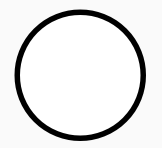
\includegraphics[width=.9\linewidth]{./pic/circle.png}

\begin{minted}[frame=lines,fontsize=\scriptsize,linenos=false]{xml}
<shape xmlns:android="http://schemas.android.com/apk/res/android"
android:shape="oval">
<stroke
    android:width="4dp"
    android:color="@android:color/black" />
<solid android:color="@android:color/white" />
</shape>
\end{minted}
\subsection{Which image best corresponds to the following LinearLayout?}
\label{sec-13-1-3}
\begin{minted}[frame=lines,fontsize=\scriptsize,linenos=false]{xml}
  <LinearLayout
      android:layout_width="match_parent"
      android:layout_height="match_parent"
      android:orientation="horizontal"
      android:gravity="center">
    <Button
        android:layout_width="wrap_content"
        android:layout_height="wrap_content"
        android:text="Button" />
    <Button
        android:layout_width="wrap_content"
        android:layout_height="wrap_content"
        android:text="Button" />
  </LinearLayout>
\end{minted}
\begin{itemize}
\item gravity="center"是描述的竖直方向上位于中间,而水平方向上同样也是位于中间,每个键的宽度由自身内容的宽度决定
\item gravity: todo
\end{itemize}
\subsection{Which code snippet would achieve the layout displayed below?}
\label{sec-13-1-4}
\begin{minted}[frame=lines,fontsize=\scriptsize,linenos=false]{java}
<androidx.constraintlayout.widget.ConstraintLayout
    ...>

    <TextView
        android:id="@+id/text_dashboard"
        android:layout_width="match_parent"
        android:layout_height="wrap_content"
        android:layout_marginStart="8dp"
        android:layout_marginEnd="8dp"
        android:textAlignment="center"
        android:text="Dashboard"
        app:layout_constraintEnd_toEndOf="parent"
        app:layout_constraintStart_toStartOf="parent"
        app:layout_constraintTop_toTopOf="parent" />

</androidx.constraintlayout.widget.ConstraintLayout>
\end{minted}
\begin{itemize}
\item 左右各留8dp,文字中间对齐;文本框高度由自身高度决定;文本框宽度拉伸match$_{\text{parent}}$;
\end{itemize}

\subsection{实现矩形,右下角白色,左上角黑色的渐变效果}
\label{sec-13-1-5}
\begin{minted}[frame=lines,fontsize=\scriptsize,linenos=false]{xml}
  <shape xmlns:android-"http://schemas.android.com/apk/res/android"
  android:shape-"rectangle">
  <gradient
      android:startColor-"@android:color/white"
      android:endColor-"@android:color/black"
      android:angle-"135"/>
    </shape>
\end{minted}
\subsection{Given the following dimens.xml file, how would you define an ImageView with medium spacing at the bottom?}
\label{sec-13-1-6}
\begin{minted}[frame=lines,fontsize=\scriptsize,linenos=false]{xml}
<?xml version=1.0 encoding="utf-8"?>
<resources>
    <dimen name="spacing_medium">8dp</dimen>
    <dimen name="spacing_large">12dp</dimen>
</resources>
\end{minted}
\begin{minted}[frame=lines,fontsize=\scriptsize,linenos=false]{xml}
<ImageView
   android:id=@+id/image_map_pin"
   android:layout_width="wrap_content"
   android:layout_heignt="wrap_content"
   android:layout_marginBottom="@dimen/spacing_medium"
   android:src=@drawable/map_pin />
\end{minted}
\subsection{You want to provide a different drawable for devices that are in landscape mode and whose language is set to French. which directory is named correctly?}
\label{sec-13-1-7}
\begin{itemize}
\item drawable-fr-land
\end{itemize}

\subsection{What folder should you use for your app's launcher icons?}
\label{sec-13-1-8}
\begin{itemize}
\item /mipmap
\end{itemize}
\section{permissions}
\label{sec-13-2}
\subsection{写外部存储权限}
\label{sec-13-2-1}
\begin{minted}[frame=lines,fontsize=\scriptsize,linenos=false]{java}
<uses-permission
     android:name="android.permission.WRITE_EXTERNAL_STORAGE"
     android:maxSdkVersion="18" />
\end{minted}
\subsection{When would you use the ActivityCompat.shouldShowRequestPermissionRationale() function?}
\label{sec-13-2-2}
\begin{minted}[frame=lines,fontsize=\scriptsize,linenos=false]{java}
ActivityCompat.shouldShowRequestPermissionRationale();
\end{minted}
\begin{itemize}
\item when a user has previously denied the request for a given permission and selected "Don't ask again," but you need the permission for your app to function
\end{itemize}

\subsection{Why might you need to include the following permission to your app?}
\label{sec-13-2-3}
\begin{minted}[frame=lines,fontsize=\scriptsize,linenos=false]{java}
android.permission.ACCESS_NETWORK_STATE
\end{minted}
\begin{itemize}
\item to monitor the network state of the devices so that you don't attempt to make network calls when the network is unavailable
\end{itemize}


\chapter{annotation}
\label{sec-14}
\section{@VisibleForTesting:}
\label{sec-14-1}
\begin{itemize}
\item to denote that a class, methos, or field has its visibility relaxed to make code testable
\end{itemize}


\chapter{apk}
\label{sec-15}
\section{basic}
\label{sec-15-1}
\subsection{When would you use a product flavour in your build setup?}
\label{sec-15-1-1}
when you want to provide different version of your app with custom configuration and resources
\subsection{To shrink your code in release builds, what tool does Android Studio use?}
\label{sec-15-1-2}
\begin{itemize}
\item R8
\end{itemize}
\section{build configuration}
\label{sec-15-2}
\subsection{Which statement, in build.gradle file, correctly denotes that the corresponding module is an Android library module?}
\label{sec-15-2-1}
\begin{minted}[frame=lines,fontsize=\scriptsize,linenos=false]{java}
 apply plugin: 'com.android.library'
\end{minted}
\subsection{You would like to enable analytics tracking only in release builds. How can you create a new field in the generated BuildConfig class to store that value?}
\label{sec-15-2-2}
\begin{minted}[frame=lines,fontsize=\scriptsize,linenos=false]{java}
buildTypes {
    debug {
        buildConfigField 'boolean', 'ENABLE_ANALYTICS', 'false'
    }
    release {
        buildConfigField 'boolean', 'ENABLE_ANALYTICS', 'true'
    }
}
\end{minted}
\subsection{To optimize your APK size, what image codec should you use?}
\label{sec-15-2-3}
\begin{itemize}
\item WebP (Reference)
\end{itemize}

\subsection{Given an APK named app-internal-debug.apk produced from the build process, which statement is likely to be true?}
\label{sec-15-2-4}
\begin{itemize}
\item This APK is created from the debug build type and internal product flavor.
\end{itemize}
\section{build errors}
\label{sec-15-3}
\subsection{When attempting to build your project, what might the following error indicate?}
\label{sec-15-3-1}
\begin{minted}[frame=lines,fontsize=\scriptsize,linenos=false]{java}
Conversion to Dalvik format filed: Unable to execute dex: method ID not in [0, 0xffff]: 65536
\end{minted}
\begin{itemize}
\item You have exceeded the total number of methods that can be referenced within a single DEX file.
\end{itemize}

\chapter{testing}
\label{sec-16}
\section{Why do you use the AndroidJUnitRunner when running UI tests?}
\label{sec-16-1}
\begin{itemize}
\item Notice: AndroidJUnitRunner lets us run JUnit3/4-style tests on Android Devices
\begin{itemize}
\item The test runner facilitates loading your test package and the app under test onto a device or emulator, runs the test, and reports the results.
\end{itemize}
\end{itemize}
\section{Given the test class below, which code snippet would be a correct assertion?}
\label{sec-16-2}
\begin{minted}[frame=lines,fontsize=\scriptsize,linenos=false]{java}
 assertNotNull(resultAdd)
\end{minted}


\chapter{debugging}
\label{sec-17}
\section{network}
\label{sec-17-1}
\subsection{You have built code to make a network call and tested that it works in your development environment. However, when you publish it to the Play console, the networking call fails to work. What will NOT help you troubleshoot this issue?}
\label{sec-17-1-1}
\begin{itemize}
\item checking whether ProGuard -keepclassmembers have been added to the network data transfer objects (DTOs) in question
\item checking for exceptions in the server logs or server console
\item checking that the network data transfer object has @SerizlizedName applied to its member properties
\item using the profiler tools in Android Studio to detect anomalies in CPU, memory, and network usage (ANSWER: this does not help)
\end{itemize}


\chapter{Frameworks}
\label{sec-18}
\section{Retrofit}
\label{sec-18-1}
\subsection{You need to remove an Event based on it;s id from your API, Which code snippet defines that request in Retrofit?}
\label{sec-18-1-1}
\begin{itemize}
\item @DELETE("events/\{id\}") fun deleteEvent(@Path("id") id: Long): Call
\end{itemize}
\subsection{You need to retrieve a list of photos from an API. Which code snippet defines an HTML GET request in Retrofit?}
\label{sec-18-1-2}
\begin{minted}[frame=lines,fontsize=\scriptsize,linenos=false]{java}
 @GET("photo") fun listPhotos() : Call<List>
\end{minted}


\chapter{需要分类出去的}
\label{sec-19}
\subsection{What are the permission protection levels in Android?}
\label{sec-19-0-1}
\begin{itemize}
\item Normal — A lower-risk permission that gives requesting applications access to isolated application-level features, with minimal risk to other applications, the system, or the user. The system automatically grants this type of permission to a requesting application at installation, without asking for the user’s explicit approval.
\item Dangerous — A higher-risk permission. Any dangerous permissions requested by an application may be displayed to the user and require confirmation before proceeding, or some other approach may be taken to avoid the user automatically allowing the use of such facilities.
\item Signature — A permission that the system grants only if the requesting application is signed with the same certificate as the application that declared the permission. If the certificates match, the system automatically grants the permission without notifying the user or asking for the user’s explicit approval.
\item SignatureOrSystem — A permission that the system grants only to applications that are in the Android system image or that are signed with the same certificate as the application that declared the permission.
\end{itemize}

\subsection{What is Android Data Binding?}
\label{sec-19-0-2}

The Data Binding Library is a support library that allows you to bind UI components in your layouts to data sources in your app using a declarative format rather than programmatically.

Layouts are often defined in activities with code that calls UI framework methods. For example, the code below calls findViewById() to find a TextView widget and bind it to the userName property of the viewModel variable:

\begin{minted}[frame=lines,fontsize=\scriptsize,linenos=false]{java}
TextView textView = findViewById(R.id.sample_text);
textView.setText(viewModel.getUserName());
\end{minted}

The following example shows how to use the Data Binding Library to assign text to the widget directly in the layout file. This removes the need to call any of the Java code shown above.

\begin{minted}[frame=lines,fontsize=\scriptsize,linenos=false]{java}
<TextView
    android:text="@{viewmodel.userName}" />
\end{minted}

\begin{itemize}
\item The pros of using Android Data Binding:
\begin{itemize}
\item Reduces boilerplate code which in turns brings
\item Less coupling
\item Stronger readability
\item Powerful, easy to implement custom attribute and custom view
\item Even faster than findViewById - The binding does a single pass on the View hierarchy, extracting the Views with IDs. This mechanism can be faster than calling findViewById for several Views.
\end{itemize}
\end{itemize}

\subsection{What is the ViewHolder pattern? Why should we use it?}
\label{sec-19-0-3}

Every time when the adapter calls getView() method, the findViewById() method is also called. This is a very intensive work for the mobile CPU and so affects the performance of the application and the battery consumption increases. ViewHolder is a design pattern which can be applied as a way around repeated use of findViewById().

A ViewHolder holds the reference to the id of the view resource and calls to the resource will not be required after you "find" them: Thus performance of the application increases.
\begin{minted}[frame=lines,fontsize=\scriptsize,linenos=false]{java}
private static class ViewHolder {
    final TextView text;
    final TextView timestamp;
    final ImageView icon;
    final ProgressBar progress;

    ViewHolder(TextView text, TextView timestamp, ImageView icon, ProgressBar progress) {
        this.text = text;
        this.timestamp = timestamp;
        this.icon = icon;
        this.progress = progress;
    }
}
public View getView(int position, View convertView, ViewGroup parent) {
    View view = convertView;
    if (view == null) {
        view = // inflate new view
        ViewHolder holder = createViewHolderFrom(view);
        view.setTag(holder);  
    }
    ViewHolder holder = view.getTag();
    // TODO: set correct data for this list item
    // holder.icon.setImageDrawable(...)
    // holder.text.setText(...)
    // holder.timestamp.setText(...)
    // holder.progress.setProgress(...)
    return view;
}
private ViewHolder createViewHolderFrom(View view) {
    ImageView icon = (ImageView) view.findViewById(R.id.listitem_image);
    TextView text = (TextView) view.findViewById(R.id.listitem_text);
    TextView timestamp = (TextView) view.findViewById(R.id.listitem_timestamp);
    ProgressBar progress = (ProgressBar) view.findViewById(R.id.progress_spinner);
    return new ViewHolder(text, timestamp, icon, progress);
}
\end{minted}
\begin{itemize}
\item View.setTag(Object) allows you to tell the View to hold an arbitrary object. If we use it to hold an instance of our ViewHolder after we do our findViewById(int) calls, then we can use View.getTag() on recycled views to avoid having to make the calls again and again.
\end{itemize}

\subsection{What is the difference between Handler vs AsyncTask vs Thread?}
\label{sec-19-0-4}
Mid 
Top 113 Android Interview Questions  Android  113  
Answer
The Handler class can be used to register to a thread and provides a simple channel to send data to this thread. A Handler allows you communicate back with the UI thread from other background thread.
The AsyncTask class encapsulates the creation of a background process and the synchronization with the main thread. It also supports reporting progress of the running tasks.
And a Thread is basically the core element of multithreading which a developer can use with the following disadvantage:
Handle synchronization with the main thread if you post back results to the user interface
No default for canceling the thread
No default thread pooling
No default for handling configuration changes in Android
Having Tech or Coding Interview? Check 👉 113 Android Interview Questions
Source: stackoverflow.com
\subsection{What is the difference between compileSdkVersion and targetSdkVersion?}
\label{sec-19-0-5}
Mid 
Top 113 Android Interview Questions  Android  113  
Answer
The compileSdkVersion is the version of the API the app is compiled against. This means you can use Android API features included in that version of the API (as well as all previous versions, obviously). If you try and use API 16 features but set compileSdkVersion to 15, you will get a compilation error. If you set compileSdkVersion to 16 you can still run the app on a API 15 device as long as your app's execution paths do not attempt to invoke any APIs specific to API 16.

The targetSdkVersion has nothing to do with how your app is compiled or what APIs you can utilize. The targetSdkVersion is supposed to indicate that you have tested your app on (presumably up to and including) the version you specify. This is more like a certification or sign off you are giving the Android OS as a hint to how it should handle your app in terms of OS features.
\subsection{What is the difference between a Bundle and an Intent?}
\label{sec-19-0-6}
Mid 
Top 113 Android Interview Questions  Android  113  
Answer
A Bundle is a collection of key-value pairs.
However, an Intent is much more. It contains information about an operation that should be performed. This new operation is defined by the action it can be used for, and the data it should show/edit/add. The system uses this information for finding a suitable app component (activity/broadcast/service) for the requested action.
Think of the Intent as a Bundle that also contains information on who should receive the contained data, and how it should be presented.

\subsection{What are the wake locks available in android?}
\label{sec-19-0-7}
A - PARTIAL$_{\text{WAKE}}$$_{\text{LOCK}}$
B - SCREEN$_{\text{DIM}}$$_{\text{WAKE}}$$_{\text{LOCK}}$
C - SCREEN$_{\text{BRIGHT}}$$_{\text{WAKE}}$$_{\text{LOCK}}$
D - FULL$_{\text{WAKE}}$$_{\text{LOCK}}$
E - FULL$_{\text{WAKE}}$$_{\text{LOCK}}$
Answer : E
Explanation
When CPU is on mode, PARTIAL$_{\text{WAKE}}$$_{\text{LOCK}}$ will be active.

When CPU + bright Screen low is on mode, SCREEN$_{\text{DIM}}$$_{\text{WAKE}}$$_{\text{LOCK}}$ will be active.

When CPU + bright Screen High is on mode,SCREEN$_{\text{BRIGHT}}$$_{\text{WAKE}}$$_{\text{LOCK}}$ will be active.

When CPU, Screen, bright Screen High is on mode, FULL$_{\text{WAKE}}$$_{\text{LOCK}}$ will be active.


\chapter{项目中用到的小点}
\label{sec-20}
\section{api level 28, androidx之前的最后一个版本}
\label{sec-20-1}

\section{android api level 30 androidx 中项目一定需要修改的条款: androidx.fragment还没有弄通}
\label{sec-20-2}
\subsection{gradles.propertiess}
\label{sec-20-2-1}
\begin{minted}[frame=lines,fontsize=\scriptsize,linenos=false]{xm}
android.useAndroidX=true
landroid.enableJetifier=true
\end{minted}
\subsection{project build.gragle: gragle versions}
\label{sec-20-2-2}
\subsection{app module build.gradle}
\label{sec-20-2-3}
\begin{minted}[frame=lines,fontsize=\scriptsize,linenos=false]{.gradle}
   implementation 'androidx.appcompat:appcompat:1.1.0'
    //implementation 'com.android.support:appcompat-v7:30.0.0'
    implementation 'com.android.support.constraint:constraint-layout:2.0.4'
    implementation 'com.android.support:design:30.0.0'
    testImplementation 'junit:junit:4.12'
    androidTestImplementation 'com.android.support.test:runner:1.0.2'
    androidTestImplementation 'com.android.support.test.espresso:espresso-core:3.0.2'
\end{minted}
\begin{itemize}
\item 什么是Jetifier? 例如,要使用androidx打包的依赖项创建新项目,此新项目需要在gradle.properties文件中添加以下行:
\end{itemize}
\subsection{JavaVersion.VERSION$_{\text{1}}$$_{\text{8}}$}
\label{sec-20-2-4}
\begin{minted}[frame=lines,fontsize=\scriptsize,linenos=false]{java}
java version 8
 compileOptions {
        sourceCompatibility JavaVersion.VERSION_1_8
        targetCompatibility JavaVersion.VERSION_1_8
    }
\end{minted}
\subsection{references}
\label{sec-20-2-5}
\begin{minted}[frame=lines,fontsize=\scriptsize,linenos=false]{java}
import android.content.Context;
import android.os.Bundle;
import android.util.Log;
import android.view.LayoutInflater;
import android.view.View;
import android.view.ViewGroup;
import android.view.Menu;
import android.view.MenuItem;
import androidx.fragment.app.Fragment;
import androidx.annotation.Nullable;
import androidx.appcompat.app.AppCompatActivity;
import androidx.appcompat.widget.Toolbar;
import android.support.design.widget.FloatingActionButton;
import android.support.design.widget.Snackbar;
import com.google.android.material.floatingactionbutton.FloatingActionButton;
import com.google.android.material.snackbar.Snackbar;
\end{minted}
\subsection{xml中也还有一些注意事项}
\label{sec-20-2-6}
\begin{minted}[frame=lines,fontsize=\scriptsize,linenos=false]{xml}
<com.me.generalprac.CustomTitleView
    android:layout_width="match_parent"
    android:layout_height="wrap_content"/>
<include layout="@layout/custom_title"/>
\end{minted}
% Emacs 27.1 (Org mode 8.2.7c)
\end{document}